\documentclass[natbib]{sigplanconf}

%\usepackage{pdfsync}
\usepackage{color}
\usepackage{graphicx}
 
%\usepackage{amsmath}
\usepackage{tikz}
%\usepackage{pgflibraryarrows}
%\usetikzlibrary{arrows}
%\newcommand{\todo}[1]{}
\newcommand{\todo}[1]{%\error                uncomment to make sure there are no todos left
 \textcolor{blue}{\mbox{$^\ast$}}\marginpar{\raggedright
 \hspace{0pt}\sffamily\tiny{\sc \textcolor{blue}{todo:}}\\ \textcolor{blue}{#1}}}
\newcommand{\bruno}[1]{\textcolor{red}{\textbf{Bruno:}#1}}
\newcommand{\alberto}[1]{\textcolor{red}{\textbf{Alberto: }#1}}
\newcommand{\btext}[1]{\textcolor{blue}{#1}}
\newcommand{\marcos}[1]{\textcolor{red}{\textbf{Marcos:}#1}}
\renewcommand{\bruno}[1]{}
\renewcommand{\alberto}[1]{}
\renewcommand{\marcos}[1]{}

%% ODER: format ==         = "\mathrel{==}"
%% ODER: format /=         = "\neq "
%
%
\makeatletter
\@ifundefined{lhs2tex.lhs2tex.sty.read}%
  {\@namedef{lhs2tex.lhs2tex.sty.read}{}%
   \newcommand\SkipToFmtEnd{}%
   \newcommand\EndFmtInput{}%
   \long\def\SkipToFmtEnd#1\EndFmtInput{}%
  }\SkipToFmtEnd

\newcommand\ReadOnlyOnce[1]{\@ifundefined{#1}{\@namedef{#1}{}}\SkipToFmtEnd}
\usepackage{amstext}
\usepackage{amssymb}
\usepackage{stmaryrd}
\DeclareFontFamily{OT1}{cmtex}{}
\DeclareFontShape{OT1}{cmtex}{m}{n}
  {<5><6><7><8>cmtex8
   <9>cmtex9
   <10><10.95><12><14.4><17.28><20.74><24.88>cmtex10}{}
\DeclareFontShape{OT1}{cmtex}{m}{it}
  {<-> ssub * cmtt/m/it}{}
\newcommand{\texfamily}{\fontfamily{cmtex}\selectfont}
\DeclareFontShape{OT1}{cmtt}{bx}{n}
  {<5><6><7><8>cmtt8
   <9>cmbtt9
   <10><10.95><12><14.4><17.28><20.74><24.88>cmbtt10}{}
\DeclareFontShape{OT1}{cmtex}{bx}{n}
  {<-> ssub * cmtt/bx/n}{}
\newcommand{\tex}[1]{\text{\texfamily#1}}	% NEU

\newcommand{\Sp}{\hskip.33334em\relax}


\newcommand{\Conid}[1]{\mathit{#1}}
\newcommand{\Varid}[1]{\mathit{#1}}
\newcommand{\anonymous}{\kern0.06em \vbox{\hrule\@width.5em}}
\newcommand{\plus}{\mathbin{+\!\!\!+}}
\newcommand{\bind}{\mathbin{>\!\!\!>\mkern-6.7mu=}}
\newcommand{\rbind}{\mathbin{=\mkern-6.7mu<\!\!\!<}}% suggested by Neil Mitchell
\newcommand{\sequ}{\mathbin{>\!\!\!>}}
\renewcommand{\leq}{\leqslant}
\renewcommand{\geq}{\geqslant}
\usepackage{polytable}

%mathindent has to be defined
\@ifundefined{mathindent}%
  {\newdimen\mathindent\mathindent\leftmargini}%
  {}%

\def\resethooks{%
  \global\let\SaveRestoreHook\empty
  \global\let\ColumnHook\empty}
\newcommand*{\savecolumns}[1][default]%
  {\g@addto@macro\SaveRestoreHook{\savecolumns[#1]}}
\newcommand*{\restorecolumns}[1][default]%
  {\g@addto@macro\SaveRestoreHook{\restorecolumns[#1]}}
\newcommand*{\aligncolumn}[2]%
  {\g@addto@macro\ColumnHook{\column{#1}{#2}}}

\resethooks

\newcommand{\onelinecommentchars}{\quad-{}- }
\newcommand{\commentbeginchars}{\enskip\{-}
\newcommand{\commentendchars}{-\}\enskip}

\newcommand{\visiblecomments}{%
  \let\onelinecomment=\onelinecommentchars
  \let\commentbegin=\commentbeginchars
  \let\commentend=\commentendchars}

\newcommand{\invisiblecomments}{%
  \let\onelinecomment=\empty
  \let\commentbegin=\empty
  \let\commentend=\empty}

\visiblecomments

\newlength{\blanklineskip}
\setlength{\blanklineskip}{0.66084ex}

\newcommand{\hsindent}[1]{\quad}% default is fixed indentation
\let\hspre\empty
\let\hspost\empty
\newcommand{\NB}{\textbf{NB}}
\newcommand{\Todo}[1]{$\langle$\textbf{To do:}~#1$\rangle$}

\EndFmtInput
\makeatother
%
%
%
%
%
%
% This package provides two environments suitable to take the place
% of hscode, called "plainhscode" and "arrayhscode". 
%
% The plain environment surrounds each code block by vertical space,
% and it uses \abovedisplayskip and \belowdisplayskip to get spacing
% similar to formulas. Note that if these dimensions are changed,
% the spacing around displayed math formulas changes as well.
% All code is indented using \leftskip.
%
% Changed 19.08.2004 to reflect changes in colorcode. Should work with
% CodeGroup.sty.
%
\ReadOnlyOnce{polycode.fmt}%
\makeatletter

\newcommand{\hsnewpar}[1]%
  {{\parskip=0pt\parindent=0pt\par\vskip #1\noindent}}

% can be used, for instance, to redefine the code size, by setting the
% command to \small or something alike
\newcommand{\hscodestyle}{}

% The command \sethscode can be used to switch the code formatting
% behaviour by mapping the hscode environment in the subst directive
% to a new LaTeX environment.

\newcommand{\sethscode}[1]%
  {\expandafter\let\expandafter\hscode\csname #1\endcsname
   \expandafter\let\expandafter\endhscode\csname end#1\endcsname}

% "compatibility" mode restores the non-polycode.fmt layout.

\newenvironment{compathscode}%
  {\par\noindent
   \advance\leftskip\mathindent
   \hscodestyle
   \let\\=\@normalcr
   \let\hspre\(\let\hspost\)%
   \pboxed}%
  {\endpboxed\)%
   \par\noindent
   \ignorespacesafterend}

\newcommand{\compaths}{\sethscode{compathscode}}

% "plain" mode is the proposed default.
% It should now work with \centering.
% This required some changes. The old version
% is still available for reference as oldplainhscode.

\newenvironment{plainhscode}%
  {\hsnewpar\abovedisplayskip
   \advance\leftskip\mathindent
   \hscodestyle
   \let\hspre\(\let\hspost\)%
   \pboxed}%
  {\endpboxed%
   \hsnewpar\belowdisplayskip
   \ignorespacesafterend}

\newenvironment{oldplainhscode}%
  {\hsnewpar\abovedisplayskip
   \advance\leftskip\mathindent
   \hscodestyle
   \let\\=\@normalcr
   \(\pboxed}%
  {\endpboxed\)%
   \hsnewpar\belowdisplayskip
   \ignorespacesafterend}

% Here, we make plainhscode the default environment.

\newcommand{\plainhs}{\sethscode{plainhscode}}
\newcommand{\oldplainhs}{\sethscode{oldplainhscode}}
\plainhs

% The arrayhscode is like plain, but makes use of polytable's
% parray environment which disallows page breaks in code blocks.

\newenvironment{arrayhscode}%
  {\hsnewpar\abovedisplayskip
   \advance\leftskip\mathindent
   \hscodestyle
   \let\\=\@normalcr
   \(\parray}%
  {\endparray\)%
   \hsnewpar\belowdisplayskip
   \ignorespacesafterend}

\newcommand{\arrayhs}{\sethscode{arrayhscode}}

% The mathhscode environment also makes use of polytable's parray 
% environment. It is supposed to be used only inside math mode 
% (I used it to typeset the type rules in my thesis).

\newenvironment{mathhscode}%
  {\parray}{\endparray}

\newcommand{\mathhs}{\sethscode{mathhscode}}

% texths is similar to mathhs, but works in text mode.

\newenvironment{texthscode}%
  {\(\parray}{\endparray\)}

\newcommand{\texths}{\sethscode{texthscode}}

% The framed environment places code in a framed box.

\def\codeframewidth{\arrayrulewidth}
\RequirePackage{calc}

\newenvironment{framedhscode}%
  {\parskip=\abovedisplayskip\par\noindent
   \hscodestyle
   \arrayrulewidth=\codeframewidth
   \tabular{@{}|p{\linewidth-2\arraycolsep-2\arrayrulewidth-2pt}|@{}}%
   \hline\framedhslinecorrect\\{-1.5ex}%
   \let\endoflinesave=\\
   \let\\=\@normalcr
   \(\pboxed}%
  {\endpboxed\)%
   \framedhslinecorrect\endoflinesave{.5ex}\hline
   \endtabular
   \parskip=\belowdisplayskip\par\noindent
   \ignorespacesafterend}

\newcommand{\framedhslinecorrect}[2]%
  {#1[#2]}

\newcommand{\framedhs}{\sethscode{framedhscode}}

% The inlinehscode environment is an experimental environment
% that can be used to typeset displayed code inline.

\newenvironment{inlinehscode}%
  {\(\def\column##1##2{}%
   \let\>\undefined\let\<\undefined\let\\\undefined
   \newcommand\>[1][]{}\newcommand\<[1][]{}\newcommand\\[1][]{}%
   \def\fromto##1##2##3{##3}%
   \def\nextline{}}{\) }%

\newcommand{\inlinehs}{\sethscode{inlinehscode}}

% The joincode environment is a separate environment that
% can be used to surround and thereby connect multiple code
% blocks.

\newenvironment{joincode}%
  {\let\orighscode=\hscode
   \let\origendhscode=\endhscode
   \def\endhscode{\def\hscode{\endgroup\def\@currenvir{hscode}\\}\begingroup}
   %\let\SaveRestoreHook=\empty
   %\let\ColumnHook=\empty
   %\let\resethooks=\empty
   \orighscode\def\hscode{\endgroup\def\@currenvir{hscode}}}%
  {\origendhscode
   \global\let\hscode=\orighscode
   \global\let\endhscode=\origendhscode}%

\makeatother
\EndFmtInput
%







%\setlength{\parindent}{0in}

\begin{document}

\conferenceinfo{PEPM'13,} {January 21--22, 2013, Rome, Italy.}
\CopyrightYear{2013}
\copyrightdata{978-1-4503-1842-6/13/01}

%\titlebanner{submitted to Haskell Symposium 2011}         % These are ignored unless
%\preprintfooter{version of Jul 21, 2012}     % 'preprint' option specified.

%\title{Fast Extensible Records In Haskell}
\title{Just Do It While Compiling!}
\subtitle{Fast Extensible Records In Haskell}


\authorinfo{Bruno Martinez Aguerre}
           {Instituto de Computaci\'{o}n \\ Universidad de la  Rep\'{u}blica\\ Montevideo, Uruguay}
           {brunom@fing.edu.uy}
\authorinfo{Marcos Viera}
           {Instituto de Computaci\'{o}n \\ Universidad de la  Rep\'{u}blica\\ Montevideo, Uruguay}
           {mviera@fing.edu.uy}
\authorinfo{Alberto Pardo}
           {Instituto de Computaci\'{o}n \\ Universidad de la  Rep\'{u}blica\\ Montevideo, Uruguay}
           {pardo@fing.edu.uy}
\maketitle

\begin{abstract}
The library for strongly typed heterogeneous collections HList
provides an implementation of extensible records in Haskell that needs
only a few common extensions of the language. In HList, records are
represented as linked lists of label-value pairs with a lookup
operation that is linear-time in the number of fields. In this paper,
we use type-level programming techniques to develop a more efficient
representation of extensible records for HList. We propose two
internal encodings for extensible records that improve lookup at
runtime without needing a total order on the labels. One of the
encodings performs lookup in constant time but at a cost of linear
time insertion. The other one performs lookup in logarithmic time
while preserving the fast insertion of simple linked lists. Through
staged compilation, the required slow search for a field is moved to
compile time in both cases.
\end{abstract}

\category{D.3.3}{Programming languages}{Language Constructs and Features}
\category{D.1.1}{Programming techniques}{Applicative (Functional) Programming}
\terms Design, Languages, Performance

\keywords
 Extensible Records, Type-level programming, Staged Computation, Haskell, HList, Balanced Trees 

\section{Introduction} \label{sec:intro}

Although there have been many different proposals for Extensible Records in Haskell 
\cite{Gaster96apolymorphic, Jones99lightweightextensible, LabeledFunctions, Leijen:fclabels, Leijen:scopedlabels, Jel10},
it is still an open problem to find an implementation that manipulates records with satisfactory efficiency.
Imperative dynamic languages use hash tables for objects,
achieving constant time insertion and lookup.
%\marcos{esto es algo que sabemos o sospechamos? hay referencias para dar?}
%\bruno{sabemos pero no encuentro mejor referencia que http://en.wikipedia.org/wiki/Hashtable}
%\marcos{hash tables heterogeneas?}
%\bruno{heterogeneas, si, porque son lenguajes dinamicos}
Inserting a field changes the table in place,
destructing the old version of the object,
not allowing for persistency as required in functional languages.
Copying the underlying array of the hash table
to preserve the old version makes insertion slower.

Clojure \cite{Hickey:2008:CPL:1408681.1408682} implements vectors with trees of small contiguous arrays,
so insertion is logarithmic due to structural sharing. 
Clojure's hash map, built on top of vectors,
then achieves logarithmic time insertion and lookup.

The usual strategies for record insertion in functional languages are
copying all existing fields along with the new one to a brand new tuple,
or using a linked list \cite{Gaster96apolymorphic}.
The tuple strategy offers the fastest possible lookup, but insertion is linear time.
The linked list sits in opposite in the tradeoff curve,
with constant time insertion but linear time lookup.
Since a record is essentially a dictionary,
the obvious strategy to bridge this gap is a search tree.
While lookup is much improved to logarithmic time,
insertion is also hit and rendered logarithmic.

Hash maps and ordered trees need hashing and compare functions.
This ends up being the biggest turnoff for these techniques in our setting.
Types, standing as field labels, do not have natural, readily accessible implementations
for these functions.

This paper aims to contribute a solution in that direction. 
Our starting point is the Haskell library for strongly typed heterogeneous collections HList \cite{KLS04}
which provides an example implementation of extensible records. 
A drawback of HList is that lookup, the most used operation on records, is linear time.
We propose two alternative implementations for extensible records as a Haskell library, using the same techniques as HList.
One, called \ensuremath{\Conid{ArrayRecord}}, uses an array to hold the fields, achieving constant time lookup but linear time insertion.
The other alternative, called \ensuremath{\Conid{SkewRecord}}, is based on a balanced tree structure. It maintains constant time insertions, but lowers lookup to logarithmic time.
%\marcos{no se habla de la version Array} \bruno{ahora si}

Another contribution of this paper is the trick we use to reduce the run time work.
We have observed that, when looking-up an element in a HList,
the element is first searched at compile time in order to determine whether it
belongs to the list.
%and raise an error when it does not.
This search generates the path the program follows at run time to obtain the element.
In Figure~\ref{fig:search-hlist} we represent with a dashed arrow the compile time search, 
and with a solid arrow the generated path followed at run time. 
Since the structure is linear, the search and the path have the same length.

\begin{figure}[tp]
\begin{center}
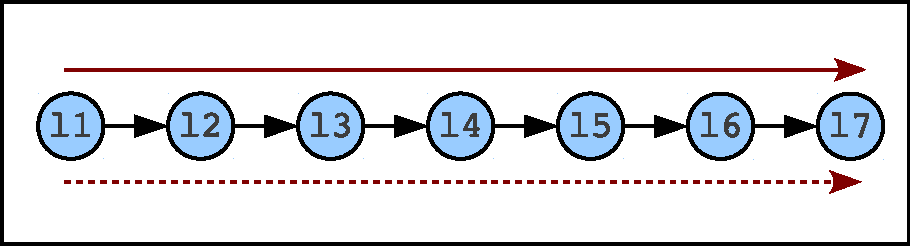
\includegraphics[scale=0.5]{search-hlist.pdf}
\end{center}
\caption{Search \ensuremath{\Varid{l7}} in HList} \label{fig:search-hlist}
\end{figure}

Thus, the key idea is very simple. When in Haskell we compare, for example, two stings, such as \ensuremath{\text{\tt \char34 foo\char34}\equiv \text{\tt \char34 baar\char34}}, the entire process of searching the correct instance of \ensuremath{\Conid{Eq}} to be used is performed at compile time. No work is done at run time to search the correct instance and discard the incorrect ones. We apply the same concept to perform the search of a label into a record. Given that a label is represented by a singleton type we have enough information to determine the ``path of instances" that goes to it, discarding any possible wrong path.
We also make use of lazy evaluation, to tell the compiler which path to follow without any cost at run time.

%Instead of a linear structure as used by HList, 
For example, one of our proposed implementations uses an alternative structure for the representation of heterogeneous collections which is based on balanced trees.
Such a structure better profits from the information given by the compile time search, leading to logarithmic length paths in the run time traversal (see Figure~\ref{fig:search-skew}). 
We show experimental results that confirm this behaviour. 

\begin{figure}[tp]
\begin{center}
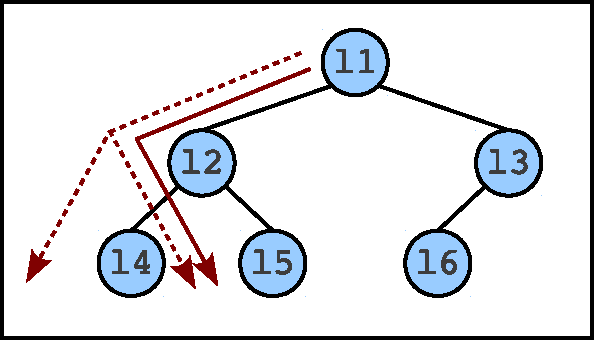
\includegraphics[scale=0.5]{search-skew.pdf}
\end{center}
\caption{Search \ensuremath{\Varid{l7}} in balanced tree} \label{fig:search-skew}
\end{figure}


The rest of the paper is organized as follows. 
We start with a brief review of the type-level techniques used to implement extensible records 
by HList (Section~\ref{sec:hlist}). 
In Section~\ref{sec:faster} we show how using the same type-level techniques we can obtain alternative implementations of extensible records with faster lookup operations at run time. 
Section~\ref{sec:efficiency} presents some experimental results that compare the implementations we propose with HList, both at compile time and run time. 
Finally, in Section~\ref{sec:conclusions} we draw some conclusions and present possible directions for future work.



\section{HList}\label{sec:hlist}

HList is a Haskell library that implements typeful heterogeneous collections, 
such as heterogeneous lists or records, using extensions of Haskell for multi-parameter 
classes \cite{PJM97} and functional dependencies \cite{Jon00}.
HList strongly relies on \emph{type-level programming} techniques by means of which
types are used to represent type-level values, and classes are used to represent 
type-level functions.

We illustrate the use of type-level programming by means of two simple examples that
will be used later in the paper. We start with a type-level representation of booleans values. 
Since we are only interested in type-level computations, we define empty 
types \ensuremath{\Conid{HTrue}} and \ensuremath{\Conid{HFalse}} corresponding to each boolean value.

\begin{hscode}\SaveRestoreHook
\column{B}{@{}>{\hspre}l<{\hspost}@{}}%
\column{8}{@{}>{\hspre}l<{\hspost}@{}}%
\column{16}{@{}>{\hspre}l<{\hspost}@{}}%
\column{26}{@{}>{\hspre}l<{\hspost}@{}}%
\column{E}{@{}>{\hspre}l<{\hspost}@{}}%
\>[B]{}\mathbf{data}\;{}\<[8]%
\>[8]{}\Conid{HTrue}{}\<[16]%
\>[16]{};\Varid{hTrue}{}\<[26]%
\>[26]{}\mathrel{=}\bot \mathbin{::}\Conid{HTrue}{}\<[E]%
\\
\>[B]{}\mathbf{data}\;{}\<[8]%
\>[8]{}\Conid{HFalse}{}\<[16]%
\>[16]{};\Varid{hFalse}{}\<[26]%
\>[26]{}\mathrel{=}\bot \mathbin{::}\Conid{HFalse}{}\<[E]%
\ColumnHook
\end{hscode}\resethooks

The inhabitants \ensuremath{\Varid{hTrue}} and \ensuremath{\Varid{hFalse}} of those types are defined solely
to be used in value-level expressions to construct type-level values by 
referring to the types of such expressions.

Type-level functions can be described using multi-parameter classes with functional dependencies. 
For example, we can encode type-level negation by defining the following class:
\begin{hscode}\SaveRestoreHook
\column{B}{@{}>{\hspre}l<{\hspost}@{}}%
\column{3}{@{}>{\hspre}l<{\hspost}@{}}%
\column{E}{@{}>{\hspre}l<{\hspost}@{}}%
\>[B]{}\mathbf{class}\;\Conid{HNot}\;\Varid{t}\;\Varid{t'}\mid \Varid{t}\to \Varid{t'}\;\mathbf{where}{}\<[E]%
\\
\>[B]{}\hsindent{3}{}\<[3]%
\>[3]{}\Varid{hNot}\mathbin{::}\Varid{t}\to \Varid{t'}{}\<[E]%
\ColumnHook
\end{hscode}\resethooks
The functional dependency \ensuremath{\Varid{t}\to \Varid{t'}} expresses that the parameter \ensuremath{\Varid{t}}
uniquely determines the parameter \ensuremath{\Varid{t'}}. 
Therefore, once \ensuremath{\Varid{t}} is instantiated,
the instance of \ensuremath{\Varid{t'}} must be uniquely inferable by the type-system.
In other words, the relation between \ensuremath{\Varid{t}} and \ensuremath{\Varid{t'}} is actually a function.
Whereas the class definition describes the type signature of the type-level function, 
the function itself is defined by the following instance declarations:

\begin{hscode}\SaveRestoreHook
\column{B}{@{}>{\hspre}l<{\hspost}@{}}%
\column{16}{@{}>{\hspre}l<{\hspost}@{}}%
\column{24}{@{}>{\hspre}l<{\hspost}@{}}%
\column{32}{@{}>{\hspre}l<{\hspost}@{}}%
\column{E}{@{}>{\hspre}l<{\hspost}@{}}%
\>[B]{}\mathbf{instance}\;\Conid{HNot}\;{}\<[16]%
\>[16]{}\Conid{HFalse}\;{}\<[24]%
\>[24]{}\Conid{HTrue}\;{}\<[32]%
\>[32]{}\mathbf{where}\;\Varid{hNot}\;\anonymous \mathrel{=}\Varid{hTrue}{}\<[E]%
\\
\>[B]{}\mathbf{instance}\;\Conid{HNot}\;{}\<[16]%
\>[16]{}\Conid{HTrue}\;{}\<[24]%
\>[24]{}\Conid{HFalse}\;{}\<[32]%
\>[32]{}\mathbf{where}\;\Varid{hNot}\;\anonymous \mathrel{=}\Varid{hFalse}{}\<[E]%
\ColumnHook
\end{hscode}\resethooks
If we write the expression \ensuremath{(\Varid{hNot}\;\Varid{hFalse})}, then we know that \ensuremath{\Varid{t}} is \ensuremath{\Conid{HFalse}}. 
So, the first instance of \ensuremath{\Varid{hNot}} is selected and thus \ensuremath{\Varid{t'}} is inferred to be \ensuremath{\Conid{HTrue}}.
Observe that the computation is completely at the type-level; 
no interesting value-level computation takes place.

Another example is the type-level representation of the maybe type. 
In this case we are interested in manipulating a value-level value associated with each type constructor.

\begin{hscode}\SaveRestoreHook
\column{B}{@{}>{\hspre}l<{\hspost}@{}}%
\column{16}{@{}>{\hspre}l<{\hspost}@{}}%
\column{E}{@{}>{\hspre}l<{\hspost}@{}}%
\>[B]{}\mathbf{data}\;\Conid{HNothing}{}\<[16]%
\>[16]{}\mathrel{=}\Conid{HNothing}{}\<[E]%
\\
\>[B]{}\mathbf{data}\;\Conid{HJust}\;\Varid{e}{}\<[16]%
\>[16]{}\mathrel{=}\Conid{HJust}\;\Varid{e}\;\mathbf{deriving}\;\Conid{Show}{}\<[E]%
\ColumnHook
\end{hscode}\resethooks

We aim to construct a type-level value of the maybe type from a boolean. For this purpose
we define the following multi-parameter class. The parameter \ensuremath{\Varid{v}} specifies the type 
of the values to be contained by a \ensuremath{\Conid{HJust}}.

\begin{hscode}\SaveRestoreHook
\column{B}{@{}>{\hspre}l<{\hspost}@{}}%
\column{5}{@{}>{\hspre}l<{\hspost}@{}}%
\column{E}{@{}>{\hspre}l<{\hspost}@{}}%
\>[B]{}\mathbf{class}\;\Conid{HMakeMaybe}\;\Varid{b}\;\Varid{v}\;\Varid{m}\mid \Varid{b}\;\Varid{v}\to \Varid{m}\;\mathbf{where}{}\<[E]%
\\
\>[B]{}\hsindent{5}{}\<[5]%
\>[5]{}\Varid{hMakeMaybe}\mathbin{::}\Varid{b}\to \Varid{v}\to \Varid{m}{}\<[E]%
\\
\>[B]{}\mathbf{instance}\;\Conid{HMakeMaybe}\;\Conid{HFalse}\;\Varid{v}\;\Conid{HNothing}\;\mathbf{where}{}\<[E]%
\\
\>[B]{}\hsindent{5}{}\<[5]%
\>[5]{}\Varid{hMakeMaybe}\;\Varid{b}\;\Varid{v}\mathrel{=}\Conid{HNothing}{}\<[E]%
\\
\>[B]{}\mathbf{instance}\;\Conid{HMakeMaybe}\;\Conid{HTrue}\;\Varid{v}\;(\Conid{HJust}\;\Varid{v})\;\mathbf{where}{}\<[E]%
\\
\>[B]{}\hsindent{5}{}\<[5]%
\>[5]{}\Varid{hMakeMaybe}\;\Varid{b}\;\Varid{v}\mathrel{=}\Conid{HJust}\;\Varid{v}{}\<[E]%
\ColumnHook
\end{hscode}\resethooks

Another operation that will be of interest on this type is the one that combines 
two values of type maybe. 

\begin{hscode}\SaveRestoreHook
\column{B}{@{}>{\hspre}l<{\hspost}@{}}%
\column{5}{@{}>{\hspre}l<{\hspost}@{}}%
\column{14}{@{}>{\hspre}l<{\hspost}@{}}%
\column{E}{@{}>{\hspre}l<{\hspost}@{}}%
\>[B]{}\mathbf{class}\;\Conid{HPlus}\;\Varid{a}\;\Varid{b}\;\Varid{c}\mid \Varid{a}\;\Varid{b}\to \Varid{c}\;\mathbf{where}{}\<[E]%
\\
\>[B]{}\hsindent{5}{}\<[5]%
\>[5]{}\Varid{hPlus}\mathbin{::}\Varid{a}\to \Varid{b}\to \Varid{c}{}\<[E]%
\\
\>[B]{}\mathbf{instance}\;\Conid{HPlus}\;(\Conid{HJust}\;\Varid{a})\;\Varid{b}\;(\Conid{HJust}\;\Varid{a})\;\mathbf{where}{}\<[E]%
\\
\>[B]{}\hsindent{5}{}\<[5]%
\>[5]{}\Varid{hPlus}\;\Varid{a}\;{}\<[14]%
\>[14]{}\anonymous \mathrel{=}\Varid{a}{}\<[E]%
\\
\>[B]{}\mathbf{instance}\;\Conid{HPlus}\;\Conid{HNothing}\;\Varid{b}\;\Varid{b}\;\mathbf{where}{}\<[E]%
\\
\>[B]{}\hsindent{5}{}\<[5]%
\>[5]{}\Varid{hPlus}\;\anonymous \;{}\<[14]%
\>[14]{}\Varid{b}\mathrel{=}\Varid{b}{}\<[E]%
\ColumnHook
\end{hscode}\resethooks

\subsection{Heterogeneous Lists}

Heterogeneous lists can be represented with the data types \ensuremath{\Conid{HNil}} and \ensuremath{\Conid{HCons}},
which model the structure of lists both at the value and type level:

\begin{hscode}\SaveRestoreHook
\column{B}{@{}>{\hspre}l<{\hspost}@{}}%
\column{17}{@{}>{\hspre}l<{\hspost}@{}}%
\column{E}{@{}>{\hspre}l<{\hspost}@{}}%
\>[B]{}\mathbf{data}\;\Conid{HNil}{}\<[17]%
\>[17]{}\mathrel{=}\Conid{HNil}{}\<[E]%
\\
\>[B]{}\mathbf{data}\;\Conid{HCons}\;\Varid{e}\;\Varid{l}{}\<[17]%
\>[17]{}\mathrel{=}\Conid{HCons}\;\Varid{e}\;\Varid{l}{}\<[E]%
\\
\>[B]{}\mathbf{infixr}\;\mathrm{2}\mathbin{`\Conid{HCons}`}{}\<[E]%
\ColumnHook
\end{hscode}\resethooks

For example, the value \ensuremath{\Conid{HCons}\;\Conid{True}\;(\Conid{HCons}\;\text{\tt 'a'}\;\Conid{HNil})} is a heterogeneous list of type \ensuremath{\Conid{HCons}\;\Conid{Bool}\;(\Conid{HCons}\;\Conid{Char}\;\Conid{HNil})}.

\subsection{Extensible Records}
\label{sec:extensiblerecords}

Records are mappings from labels to values.
They are modeled by an \ensuremath{\Conid{HList}} containing a heterogeneous list of fields.
A field with label \ensuremath{\Varid{l}} and value of type \ensuremath{\Varid{v}} is represented by the type:

\begin{hscode}\SaveRestoreHook
\column{B}{@{}>{\hspre}l<{\hspost}@{}}%
\column{4}{@{}>{\hspre}c<{\hspost}@{}}%
\column{4E}{@{}l@{}}%
\column{9}{@{}>{\hspre}l<{\hspost}@{}}%
\column{21}{@{}>{\hspre}c<{\hspost}@{}}%
\column{21E}{@{}l@{}}%
\column{25}{@{}>{\hspre}l<{\hspost}@{}}%
\column{E}{@{}>{\hspre}l<{\hspost}@{}}%
\>[B]{}\mathbf{newtype}\;\Conid{Field}\;\Varid{l}\;\Varid{v}{}\<[21]%
\>[21]{}\mathrel{=}{}\<[21E]%
\>[25]{}\Conid{Field}\;\{\mskip1.5mu \Varid{value}\mathbin{::}\Varid{v}\mskip1.5mu\}{}\<[E]%
\\
\>[B]{}(\mathbin{.\!\!=\!\!.}){}\<[21]%
\>[21]{}\mathbin{::}{}\<[21E]%
\>[25]{}\Varid{l}\to \Varid{v}\to \Conid{Field}\;\Varid{l}\;\Varid{v}{}\<[E]%
\\
\>[B]{}\anonymous {}\<[4]%
\>[4]{}\mathbin{.\!\!=\!\!.}{}\<[4E]%
\>[9]{}\Varid{v}{}\<[21]%
\>[21]{}\mathrel{=}{}\<[21E]%
\>[25]{}\Conid{Field}\;\Varid{v}{}\<[E]%
\ColumnHook
\end{hscode}\resethooks

\noindent 
Notice that the label is a phantom type \cite{Hin03}. 
We can retrieve the label value by using the function \ensuremath{\Varid{label}}, which exposes 
the phantom type parameter:

\begin{hscode}\SaveRestoreHook
\column{B}{@{}>{\hspre}l<{\hspost}@{}}%
\column{8}{@{}>{\hspre}c<{\hspost}@{}}%
\column{8E}{@{}l@{}}%
\column{12}{@{}>{\hspre}l<{\hspost}@{}}%
\column{E}{@{}>{\hspre}l<{\hspost}@{}}%
\>[B]{}\Varid{label}{}\<[8]%
\>[8]{}\mathbin{::}{}\<[8E]%
\>[12]{}\Conid{Field}\;\Varid{l}\;\Varid{v}\to \Varid{l}{}\<[E]%
\\
\>[B]{}\Varid{label}{}\<[8]%
\>[8]{}\mathrel{=}{}\<[8E]%
\>[12]{}\bot {}\<[E]%
\ColumnHook
\end{hscode}\resethooks

We define separate types and constructors for labels.

\begin{hscode}\SaveRestoreHook
\column{B}{@{}>{\hspre}l<{\hspost}@{}}%
\column{E}{@{}>{\hspre}l<{\hspost}@{}}%
\>[B]{}\mathbf{data}\;\Conid{L1}\mathrel{=}\Conid{L1}{}\<[E]%
\\
\>[B]{}\mathbf{data}\;\Conid{L2}\mathrel{=}\Conid{L2}{}\<[E]%
\\
\>[B]{}\mathbf{data}\;\Conid{L3}\mathrel{=}\Conid{L3}{}\<[E]%
\\
\>[B]{}\mathbf{data}\;\Conid{L4}\mathrel{=}\Conid{L4}{}\<[E]%
\\
\>[B]{}\mathbf{data}\;\Conid{L5}\mathrel{=}\Conid{L5}{}\<[E]%
\\
\>[B]{}\mathbf{data}\;\Conid{L6}\mathrel{=}\Conid{L6}{}\<[E]%
\\
\>[B]{}\mathbf{data}\;\Conid{L7}\mathrel{=}\Conid{L7}{}\<[E]%
\ColumnHook
\end{hscode}\resethooks

Thus, the following defines a record (\ensuremath{\Varid{rList}}) with seven fields:

\begin{hscode}\SaveRestoreHook
\column{B}{@{}>{\hspre}l<{\hspost}@{}}%
\column{3}{@{}>{\hspre}l<{\hspost}@{}}%
\column{8}{@{}>{\hspre}c<{\hspost}@{}}%
\column{8E}{@{}l@{}}%
\column{13}{@{}>{\hspre}l<{\hspost}@{}}%
\column{22}{@{}>{\hspre}c<{\hspost}@{}}%
\column{22E}{@{}l@{}}%
\column{25}{@{}>{\hspre}l<{\hspost}@{}}%
\column{E}{@{}>{\hspre}l<{\hspost}@{}}%
\>[B]{}\Varid{rList}\mathrel{=}{}\<[E]%
\\
\>[B]{}\hsindent{3}{}\<[3]%
\>[3]{}(\Conid{L1}{}\<[8]%
\>[8]{}\mathbin{.\!\!=\!\!.}{}\<[8E]%
\>[13]{}\Conid{True}{}\<[22]%
\>[22]{}){}\<[22E]%
\>[25]{}\mathbin{`\Conid{HCons}`}{}\<[E]%
\\
\>[B]{}\hsindent{3}{}\<[3]%
\>[3]{}(\Conid{L2}{}\<[8]%
\>[8]{}\mathbin{.\!\!=\!\!.}{}\<[8E]%
\>[13]{}\mathrm{9}{}\<[22]%
\>[22]{}){}\<[22E]%
\>[25]{}\mathbin{`\Conid{HCons}`}{}\<[E]%
\\
\>[B]{}\hsindent{3}{}\<[3]%
\>[3]{}(\Conid{L3}{}\<[8]%
\>[8]{}\mathbin{.\!\!=\!\!.}{}\<[8E]%
\>[13]{}\text{\tt \char34 bla\char34}{}\<[22]%
\>[22]{}){}\<[22E]%
\>[25]{}\mathbin{`\Conid{HCons}`}{}\<[E]%
\\
\>[B]{}\hsindent{3}{}\<[3]%
\>[3]{}(\Conid{L4}{}\<[8]%
\>[8]{}\mathbin{.\!\!=\!\!.}{}\<[8E]%
\>[13]{}\text{\tt 'c'}{}\<[22]%
\>[22]{}){}\<[22E]%
\>[25]{}\mathbin{`\Conid{HCons}`}{}\<[E]%
\\
\>[B]{}\hsindent{3}{}\<[3]%
\>[3]{}(\Conid{L5}{}\<[8]%
\>[8]{}\mathbin{.\!\!=\!\!.}{}\<[8E]%
\>[13]{}\Conid{Nothing}{}\<[22]%
\>[22]{}){}\<[22E]%
\>[25]{}\mathbin{`\Conid{HCons}`}{}\<[E]%
\\
\>[B]{}\hsindent{3}{}\<[3]%
\>[3]{}(\Conid{L6}{}\<[8]%
\>[8]{}\mathbin{.\!\!=\!\!.}{}\<[8E]%
\>[13]{}[\mskip1.5mu \mathrm{4},\mathrm{5}\mskip1.5mu]{}\<[22]%
\>[22]{}){}\<[22E]%
\>[25]{}\mathbin{`\Conid{HCons}`}{}\<[E]%
\\
\>[B]{}\hsindent{3}{}\<[3]%
\>[3]{}(\Conid{L7}{}\<[8]%
\>[8]{}\mathbin{.\!\!=\!\!.}{}\<[8E]%
\>[13]{}\text{\tt \char34 last\char34}{}\<[22]%
\>[22]{}){}\<[22E]%
\>[25]{}\mathbin{`\Conid{HCons}`}{}\<[E]%
\\
\>[B]{}\hsindent{3}{}\<[3]%
\>[3]{}\Conid{HNil}{}\<[E]%
\ColumnHook
\end{hscode}\resethooks

The class \ensuremath{\Conid{HListGet}} retrieves from a record the value part
corresponding to a specific label:

\begin{hscode}\SaveRestoreHook
\column{B}{@{}>{\hspre}l<{\hspost}@{}}%
\column{5}{@{}>{\hspre}l<{\hspost}@{}}%
\column{E}{@{}>{\hspre}l<{\hspost}@{}}%
\>[B]{}\mathbf{class}\;\Conid{HListGet}\;\Varid{r}\;\Varid{l}\;\Varid{v}\mid \Varid{r}\;\Varid{l}\to \Varid{v}\;\mathbf{where}{}\<[E]%
\\
\>[B]{}\hsindent{5}{}\<[5]%
\>[5]{}\Varid{hListGet}\mathbin{::}\Varid{r}\to \Varid{l}\to \Varid{v}{}\<[E]%
\ColumnHook
\end{hscode}\resethooks

\noindent 
At the type-level it is statically checked that the record \ensuremath{\Varid{r}} indeed has
a field with label \ensuremath{\Varid{l}} associated with a value of the type \ensuremath{\Varid{v}}.
At value-level \ensuremath{\Varid{hListGet}} returns the value of type \ensuremath{\Varid{v}}.
For example, the following expression returns the string \ensuremath{\text{\tt \char34 last\char34}}:

\begin{hscode}\SaveRestoreHook
\column{B}{@{}>{\hspre}l<{\hspost}@{}}%
\column{E}{@{}>{\hspre}l<{\hspost}@{}}%
\>[B]{}\Varid{lastList}\mathrel{=}\Varid{hListGet}\;\Varid{rList}\;\Conid{L7}{}\<[E]%
\ColumnHook
\end{hscode}\resethooks

Instead of polluting the definitions of type-level functions
with the overlapping instance extension when comparing two types to be equal (e.g. labels),
HList encapsulates type comparison in \ensuremath{\Conid{HEq}}.
The type equality predicate \ensuremath{\Conid{HEq}} results in \ensuremath{\Conid{HTrue}} in case the compared types are equal and \ensuremath{\Conid{HFalse}} otherwise.
Thus, when comparing two types in other type-level functions (like \ensuremath{\Conid{HListGet}} below), 
these two cases can be discriminated without using overlapping instances.
\begin{hscode}\SaveRestoreHook
\column{B}{@{}>{\hspre}l<{\hspost}@{}}%
\column{E}{@{}>{\hspre}l<{\hspost}@{}}%
\>[B]{}\mathbf{class}\;\Conid{HEq}\;\Varid{x}\;\Varid{y}\;\Varid{b}\mid \Varid{x}\;\Varid{y}\to \Varid{b}{}\<[E]%
\\
\>[B]{}\Varid{hEq}\mathbin{::}\Conid{HEq}\;\Varid{x}\;\Varid{y}\;\Varid{b}\Rightarrow \Varid{x}\to \Varid{y}\to \Varid{b}{}\<[E]%
\\
\>[B]{}\Varid{hEq}\mathrel{=}\bot {}\<[E]%
\ColumnHook
\end{hscode}\resethooks
%
We will not delve into the different possible definitions for \ensuremath{\Conid{HEq}}.
For completeness, here is one that suffices for our purposes.
For a more complete discussion about type equality in Haskell
we refer to \cite{type-eq}.
\begin{hscode}\SaveRestoreHook
\column{B}{@{}>{\hspre}l<{\hspost}@{}}%
\column{25}{@{}>{\hspre}l<{\hspost}@{}}%
\column{E}{@{}>{\hspre}l<{\hspost}@{}}%
\>[B]{}\mathbf{instance}\;{}\<[25]%
\>[25]{}\Conid{HEq}\;\Varid{x}\;\Varid{x}\;\Conid{HTrue}{}\<[E]%
\\
\>[B]{}\mathbf{instance}\;\Varid{b}\mathbin{\;\sim\!}\Conid{HFalse}\Rightarrow {}\<[25]%
\>[25]{}\Conid{HEq}\;\Varid{x}\;\Varid{y}\;\Varid{b}{}\<[E]%
\ColumnHook
\end{hscode}\resethooks
At this point we can see that the use of overlapping instances is unavoidable. This explains why 
the implementation of HList is based on type classes and functional dependencies instead of \emph{type families} \cite{Chak05,1086397,Schrijvers2008} (which do not support overlapping instances). 

\ensuremath{\Conid{HListGet}} uses \ensuremath{\Conid{HEq}} to discriminate the two possible cases.
Either the label of the current field matches \ensuremath{\Varid{l}},
or the search must continue to the next node.

\begin{hscode}\SaveRestoreHook
\column{B}{@{}>{\hspre}l<{\hspost}@{}}%
\column{5}{@{}>{\hspre}l<{\hspost}@{}}%
\column{8}{@{}>{\hspre}l<{\hspost}@{}}%
\column{9}{@{}>{\hspre}l<{\hspost}@{}}%
\column{E}{@{}>{\hspre}l<{\hspost}@{}}%
\>[B]{}\mathbf{instance}{}\<[E]%
\\
\>[B]{}\hsindent{5}{}\<[5]%
\>[5]{}({}\<[8]%
\>[8]{}\Conid{HEq}\;\Varid{l}\;\Varid{l'}\;\Varid{b}{}\<[E]%
\\
\>[B]{}\hsindent{5}{}\<[5]%
\>[5]{},{}\<[8]%
\>[8]{}\Conid{HListGet'}\;\Varid{b}\;\Varid{v'}\;\Varid{r'}\;\Varid{l}\;\Varid{v})\Rightarrow {}\<[E]%
\\
\>[8]{}\Conid{HListGet}\;(\Conid{HCons}\;(\Conid{Field}\;\Varid{l'}\;\Varid{v'})\;\Varid{r'})\;\Varid{l}\;\Varid{v}\;\mathbf{where}{}\<[E]%
\\
\>[B]{}\hsindent{5}{}\<[5]%
\>[5]{}\Varid{hListGet}\;(\Conid{HCons}\;\Varid{f'}\mathord{@}(\Conid{Field}\;\Varid{v'})\;\Varid{r'})\;\Varid{l}\mathrel{=}{}\<[E]%
\\
\>[5]{}\hsindent{4}{}\<[9]%
\>[9]{}\Varid{hListGet'}\;(\Varid{hEq}\;\Varid{l}\;(\Varid{label}\;\Varid{f'}))\;\Varid{v'}\;\Varid{r'}\;\Varid{l}{}\<[E]%
\ColumnHook
\end{hscode}\resethooks
 
\ensuremath{\Conid{HListGet'}} has two instances, for the cases \ensuremath{\Conid{HTrue}} and \ensuremath{\Conid{HFalse}}.

\begin{hscode}\SaveRestoreHook
\column{B}{@{}>{\hspre}l<{\hspost}@{}}%
\column{5}{@{}>{\hspre}l<{\hspost}@{}}%
\column{E}{@{}>{\hspre}l<{\hspost}@{}}%
\>[B]{}\mathbf{class}\;\Conid{HListGet'}\;\Varid{b}\;\Varid{v'}\;\Varid{r'}\;\Varid{l}\;\Varid{v}\mid \Varid{b}\;\Varid{v'}\;\Varid{r'}\;\Varid{l}\to \Varid{v}\;\mathbf{where}{}\<[E]%
\\
\>[B]{}\hsindent{5}{}\<[5]%
\>[5]{}\Varid{hListGet'}\mathbin{::}\Varid{b}\to \Varid{v'}\to \Varid{r'}\to \Varid{l}\to \Varid{v}{}\<[E]%
\\[\blanklineskip]%
\>[B]{}\mathbf{instance}{}\<[E]%
\\
\>[B]{}\hsindent{5}{}\<[5]%
\>[5]{}\Conid{HListGet'}\;\Conid{HTrue}\;\Varid{v}\;\Varid{r'}\;\Varid{l}\;\Varid{v}{}\<[E]%
\\
\>[B]{}\hsindent{5}{}\<[5]%
\>[5]{}\mathbf{where}{}\<[E]%
\\
\>[B]{}\hsindent{5}{}\<[5]%
\>[5]{}\Varid{hListGet'}\;\anonymous \;\Varid{v}\;\anonymous \;\anonymous \mathrel{=}\Varid{v}{}\<[E]%
\\[\blanklineskip]%
\>[B]{}\mathbf{instance}{}\<[E]%
\\
\>[B]{}\hsindent{5}{}\<[5]%
\>[5]{}\Conid{HListGet}\;\Varid{r'}\;\Varid{l}\;\Varid{v}\Rightarrow {}\<[E]%
\\
\>[B]{}\hsindent{5}{}\<[5]%
\>[5]{}\Conid{HListGet'}\;\Conid{HFalse}\;\Varid{v'}\;\Varid{r'}\;\Varid{l}\;\Varid{v}\;\mathbf{where}{}\<[E]%
\\
\>[B]{}\hsindent{5}{}\<[5]%
\>[5]{}\Varid{hListGet'}\;\anonymous \;\anonymous \;\Varid{r'}\;\Varid{l}\mathrel{=}\Varid{hListGet}\;\Varid{r'}\;\Varid{l}{}\<[E]%
\ColumnHook
\end{hscode}\resethooks

\noindent
If the labels match, the corresponding value is returned, both at the value and type levels.
Otherwise, \ensuremath{\Conid{HListGet'}} calls back to \ensuremath{\Conid{HListGet}} to continue the search.  
The two type-functions are mutually recursive.  
There is no case for the empty list; lookup fails.

For GHC, the type level machinery not only generates correct value level code, 
but efficient code too.
At the value level, the functions \ensuremath{\Varid{hListGet}} and \ensuremath{\Varid{hListGet'}} are trivial,
devoid of logic and conditions.
For this reason,
GHC is smart enough to elide the dictionary objects and indirect jumps for \ensuremath{\Varid{hListGet}}.
The code is inlined to a case cascade, but the program must traverse the linked list.
For example, this is the GHC core of the example:

\begin{hscode}\SaveRestoreHook
\column{B}{@{}>{\hspre}l<{\hspost}@{}}%
\column{3}{@{}>{\hspre}l<{\hspost}@{}}%
\column{5}{@{}>{\hspre}l<{\hspost}@{}}%
\column{7}{@{}>{\hspre}l<{\hspost}@{}}%
\column{9}{@{}>{\hspre}l<{\hspost}@{}}%
\column{11}{@{}>{\hspre}l<{\hspost}@{}}%
\column{13}{@{}>{\hspre}l<{\hspost}@{}}%
\column{14}{@{}>{\hspre}l<{\hspost}@{}}%
\column{15}{@{}>{\hspre}l<{\hspost}@{}}%
\column{16}{@{}>{\hspre}l<{\hspost}@{}}%
\column{E}{@{}>{\hspre}l<{\hspost}@{}}%
\>[B]{}\Varid{lastListCore}\mathrel{=}\mathbf{case}\;\Varid{rList}\;\mathbf{of}{}\<[E]%
\\
\>[B]{}\hsindent{3}{}\<[3]%
\>[3]{}\Conid{HCons}\;\anonymous \;\Varid{rs1}\to \mathbf{case}\;\Varid{rs1}\;\mathbf{of}{}\<[E]%
\\
\>[3]{}\hsindent{2}{}\<[5]%
\>[5]{}\Conid{HCons}\;\anonymous \;{}\<[14]%
\>[14]{}\Varid{rs2}\to \mathbf{case}\;\Varid{rs2}\;\mathbf{of}{}\<[E]%
\\
\>[5]{}\hsindent{2}{}\<[7]%
\>[7]{}\Conid{HCons}\;\anonymous \;{}\<[16]%
\>[16]{}\Varid{rs3}\to \mathbf{case}\;\Varid{rs3}\;\mathbf{of}{}\<[E]%
\\
\>[7]{}\hsindent{2}{}\<[9]%
\>[9]{}\Conid{HCons}\;\anonymous \;\Varid{rs4}\to \mathbf{case}\;\Varid{rs4}\;\mathbf{of}{}\<[E]%
\\
\>[9]{}\hsindent{2}{}\<[11]%
\>[11]{}\Conid{HCons}\;\anonymous \;\Varid{rs5}\to \mathbf{case}\;\Varid{rs5}\;\mathbf{of}{}\<[E]%
\\
\>[11]{}\hsindent{2}{}\<[13]%
\>[13]{}\Conid{HCons}\;\anonymous \;\Varid{rs6}\to \mathbf{case}\;\Varid{rs6}\;\mathbf{of}{}\<[E]%
\\
\>[13]{}\hsindent{2}{}\<[15]%
\>[15]{}\Conid{HCons}\;\Varid{e}\;\anonymous \to \Varid{e}{}\<[E]%
\ColumnHook
\end{hscode}\resethooks

\section{Faster Extensible Records}\label{sec:faster}

Extensible records can double as
``static type-safe" dictionaries, that is,
collections that guarantee at compile time
that all labels searched for are available.
For example, \cite{FlyFirstClass}, a library for first-class attribute
grammars, uses extensible records to encode the collection of
attributes associated to each non-terminal. If we wanted to use it to
implement a system with a big number of attributes (e.g. a compiler)
an efficient structure would be needed.
Increasing the size of GHC's context reduction stack
makes the program compile
but at run time the linear time lookup algorithm
hurts performance.\marcos{queda medio raro esto}
The usual replacement when lookup in a linked list is slow
is a search tree.
In that case we would need to define a \ensuremath{\Conid{HOrd}} type-function
analogue to HList's magic \ensuremath{\Conid{HEq}}
and port some standard balanced tree to compile time,
tricky rotations and all.
As unappealing as this already is,
the real roadblock is \ensuremath{\Conid{HOrd}}.
Without help from the compiler,
defining such type function for
unstructured labels is beyond (our) reach. 

The key insight is that sub-linear behavior is only needed at run time.
We do not worry if the work done at compile time is superlinear
as long as it helps us to speed up our programs at run time.
\ensuremath{\Conid{HListGet}} already looks for our label at compile time
to fail compilation if we require a field for a record
without such label.
So our idea is to maintain the fields stored unordered, but
%we just store our field unordered 
in a structure that allows fast random access and depends on the compiler to
hardcode the path to our fields.

We will present two variants of faster records.
To make code listing shorter and easier to understand,
we implement each variant with independent interfaces.
However, it would be possible to provide a common class-based interface
for all variants. 

The first variant follows the conventional approach of
storing the record as a tuple.
However, because Haskell does not offer
genericity over the length of tuples as in \cite{Tullsen00thezip}, i.e. efficient access to the $i$-th element of an arbitrary length tuple,
we will use an array instead, converting field values to a common type.
%|Any| via |unsafeCoerce|,
%since array elements must be of the same type.
%Apart from this breach of type safety,
This implementation supports linear time insertions
and constant time lookups.

The second variant is tree-like, being
based on Skew Binary Random-Access Lists~\cite{OkaThesis}, a structure that guarantees constant time  insertions and logarithmic time access to any element. 
Other, perhaps simpler, data structures
such as Braun trees \cite{brauntrees} could have been chosen, since
the key property
of searching at compile time while retrieving at run time
works unchanged in any balanced tree structure.
However, those structures do not offer constant time insertion
and are not drop-in replacements for simple linear lists.
A structure with logarithmic insertion slows down
applications heavy on record modification.

\subsection{Array Records}\label{sec:array}

An Array Record has two components:
an array containing the values of the fields, and an heterogeneous list used to find a field's ordinal for lookup in the array.
To allow the storage of elements of different types in the array, we use the type \ensuremath{\Conid{Any}}\footnote{A special type that can be used as a safe placeholder for any value.}. 
Items are then \ensuremath{\Varid{unsafeCoerce}}d on the way in and out based on the type information we keep in the heterogeneous list.
%A proper implementation would hide the data constructor
%in a separate module to ensure type safety.
%\alberto{type safety o type abstraction?}
%
%
\begin{hscode}\SaveRestoreHook
\column{B}{@{}>{\hspre}l<{\hspost}@{}}%
\column{3}{@{}>{\hspre}l<{\hspost}@{}}%
\column{E}{@{}>{\hspre}l<{\hspost}@{}}%
\>[B]{}\mathbf{data}\;\Conid{ArrayRecord}\;\Varid{r}\mathrel{=}{}\<[E]%
\\
\>[B]{}\hsindent{3}{}\<[3]%
\>[3]{}\Conid{ArrayRecord}\;\Varid{r}\;(\Conid{Array}\;\Conid{Int}\;\Conid{Any}){}\<[E]%
\ColumnHook
\end{hscode}\resethooks

\subsubsection{Lookup}
Lookup is done as a two step operation.
First, the ordinal of a certain label in the record, and the type (\ensuremath{\Varid{v}}) of its stored element, are found with \ensuremath{\Conid{ArrayFind}}.
%
\begin{hscode}\SaveRestoreHook
\column{B}{@{}>{\hspre}l<{\hspost}@{}}%
\column{3}{@{}>{\hspre}l<{\hspost}@{}}%
\column{E}{@{}>{\hspre}l<{\hspost}@{}}%
\>[B]{}\mathbf{class}\;\Conid{ArrayFind}\;\Varid{r}\;\Varid{l}\;\Varid{v}\mid \Varid{r}\;\Varid{l}\to \Varid{v}\;\mathbf{where}{}\<[E]%
\\
\>[B]{}\hsindent{3}{}\<[3]%
\>[3]{}\Varid{arrayFind}\mathbin{::}\Varid{r}\to \Varid{l}\to \Conid{Int}{}\<[E]%
\ColumnHook
\end{hscode}\resethooks
%
Second, function \ensuremath{\Varid{hArrayGet}} uses the index to obtain the element from the array and the
type (\ensuremath{\Varid{v}}) to coerce that element to its correct type.
%
\begin{hscode}\SaveRestoreHook
\column{B}{@{}>{\hspre}l<{\hspost}@{}}%
\column{3}{@{}>{\hspre}l<{\hspost}@{}}%
\column{E}{@{}>{\hspre}l<{\hspost}@{}}%
\>[B]{}\Varid{hArrayGet}\mathbin{::}\Conid{ArrayFind}\;\Varid{r}\;\Varid{l}\;\Varid{v}\Rightarrow \Conid{ArrayRecord}\;\Varid{r}\to \Varid{l}\to \Varid{v}{}\<[E]%
\\
\>[B]{}\Varid{hArrayGet}\;(\Conid{ArrayRecord}\;\Varid{r}\;\Varid{a})\;\Varid{l}\mathrel{=}{}\<[E]%
\\
\>[B]{}\hsindent{3}{}\<[3]%
\>[3]{}\Varid{unsafeCoerce}\;(\Varid{a}\mathbin{!}\Varid{arrayFind}\;\Varid{r}\;\Varid{l}){}\<[E]%
\ColumnHook
\end{hscode}\resethooks

Figure~\ref{fig:search-array} shows a graphical representation of this process. 
Dashed arrow represents the compile time search of the field in the heterogeneous list which results in the index of the element in the array. Using this index the element is retrieved from the array in constant time at run time (solid arrow).

\begin{figure}[t]
\begin{center}
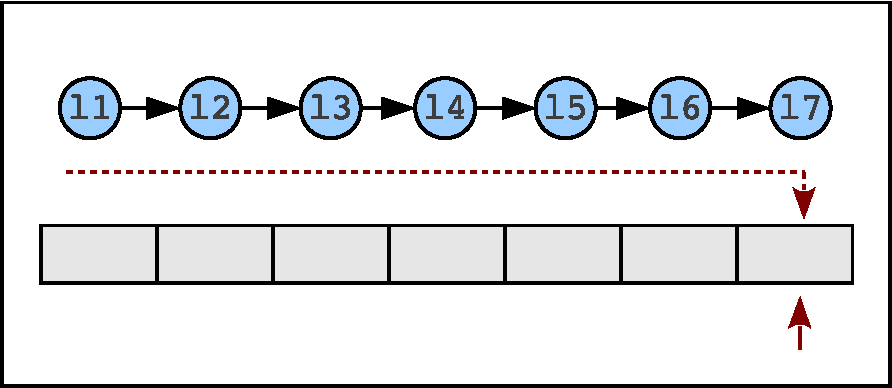
\includegraphics[scale=0.5]{search-array.pdf}
\end{center}
\caption{Search \ensuremath{\Varid{l7}} in Array} \label{fig:search-array}
\end{figure}

\ensuremath{\Conid{ArrayFind}} follows the same pattern as \ensuremath{\Conid{HListGet}} shown earlier, 
using \ensuremath{\Conid{HEq}} to discriminate the cases of 
the label of the current field, which may match or not the searched one. 
%
\begin{hscode}\SaveRestoreHook
\column{B}{@{}>{\hspre}l<{\hspost}@{}}%
\column{4}{@{}>{\hspre}l<{\hspost}@{}}%
\column{6}{@{}>{\hspre}l<{\hspost}@{}}%
\column{8}{@{}>{\hspre}l<{\hspost}@{}}%
\column{11}{@{}>{\hspre}c<{\hspost}@{}}%
\column{11E}{@{}l@{}}%
\column{14}{@{}>{\hspre}l<{\hspost}@{}}%
\column{E}{@{}>{\hspre}l<{\hspost}@{}}%
\>[B]{}\mathbf{instance}\;{}\<[11]%
\>[11]{}({}\<[11E]%
\>[14]{}\Conid{HEq}\;\Varid{l}\;\Varid{l'}\;\Varid{b}{}\<[E]%
\\
\>[11]{},{}\<[11E]%
\>[14]{}\Conid{ArrayFind'}\;\Varid{b}\;\Varid{v'}\;\Varid{r}\;\Varid{l}\;\Varid{v}\;\Varid{n}{}\<[E]%
\\
\>[11]{},{}\<[11E]%
\>[14]{}\Conid{ToValue}\;\Varid{n})\Rightarrow {}\<[E]%
\\
\>[B]{}\hsindent{4}{}\<[4]%
\>[4]{}\Conid{ArrayFind}\;(\Conid{HCons}\;(\Conid{Field}\;\Varid{l'}\;\Varid{v'})\;\Varid{r})\;\Varid{l}\;\Varid{v}\;\mathbf{where}{}\<[E]%
\\
\>[4]{}\hsindent{2}{}\<[6]%
\>[6]{}\Varid{arrayFind}\;(\Conid{HCons}\;\Varid{f}\;\Varid{r})\;\Varid{l}\mathrel{=}{}\<[E]%
\\
\>[6]{}\hsindent{2}{}\<[8]%
\>[8]{}\Varid{toValue}\;(\Varid{arrayFind'}\;(\Varid{hEq}\;\Varid{l}\;(\Varid{label}\;\Varid{f}))\;(\Varid{value}\;\Varid{f})\;\Varid{r}\;\Varid{l}){}\<[E]%
\ColumnHook
\end{hscode}\resethooks
%
A difference with \ensuremath{\Conid{HListGet}} is that the work of searching the label,
performed by \ensuremath{\Conid{ArrayFind'}}, is only done at type-level.
There is no value-level member of the class \ensuremath{\Conid{ArrayFind'}};
observe that \ensuremath{\Varid{arrayFind'}} is just an undefined value
and nothing will be computed at run time.
%
\begin{hscode}\SaveRestoreHook
\column{B}{@{}>{\hspre}l<{\hspost}@{}}%
\column{10}{@{}>{\hspre}l<{\hspost}@{}}%
\column{16}{@{}>{\hspre}l<{\hspost}@{}}%
\column{25}{@{}>{\hspre}l<{\hspost}@{}}%
\column{E}{@{}>{\hspre}l<{\hspost}@{}}%
\>[B]{}\Varid{arrayFind'}\mathbin{::}{}\<[16]%
\>[16]{}\Conid{ArrayFind'}\;\Varid{b}\;\Varid{v'}\;\Varid{r}\;\Varid{l}\;\Varid{v}\;\Varid{n}{}\<[E]%
\\
\>[16]{}\Rightarrow \Varid{b}\to \Varid{v'}\to \Varid{r}\to \Varid{l}\to \Varid{n}{}\<[E]%
\\
\>[B]{}\Varid{arrayFind'}\mathrel{=}\bot {}\<[E]%
\\[\blanklineskip]%
\>[B]{}\mathbf{data}\;\Conid{HZero}{}\<[E]%
\\
\>[B]{}\mathbf{data}\;\Conid{HSucc}\;\Varid{n}{}\<[E]%
\\[\blanklineskip]%
\>[B]{}\mathbf{class}\;\Conid{ArrayFind'}\;\Varid{b}\;\Varid{v'}\;\Varid{r}\;\Varid{l}\;\Varid{v}\;\Varid{n}\mid \Varid{b}\;\Varid{v'}\;\Varid{r}\;\Varid{l}\to \Varid{v}\;\Varid{n}{}\<[E]%
\\
\>[B]{}\mathbf{instance}\;\Conid{ArrayFind'}\;\Conid{HTrue}\;\Varid{v}\;\Varid{r}\;\Varid{l}\;\Varid{v}\;\Conid{HZero}{}\<[E]%
\\
\>[B]{}\mathbf{instance}\;(\Conid{HEq}\;\Varid{l}\;\Varid{l'}\;\Varid{b},\Conid{ArrayFind'}\;\Varid{b}\;\Varid{v'}\;\Varid{r}\;\Varid{l}\;\Varid{v}\;\Varid{n}){}\<[E]%
\\
\>[B]{}\hsindent{10}{}\<[10]%
\>[10]{}\Rightarrow \Conid{ArrayFind'}\;{}\<[25]%
\>[25]{}\Conid{HFalse}\;\Varid{v''}\;(\Conid{HCons}\;(\Conid{Field}\;\Varid{l'}\;\Varid{v'})\;\Varid{r})\;\Varid{l}\;{}\<[E]%
\\
\>[25]{}\Varid{v}\;(\Conid{HSucc}\;\Varid{n}){}\<[E]%
\ColumnHook
\end{hscode}\resethooks
%
The types \ensuremath{\Conid{HZero}} and \ensuremath{\Conid{HSucc}} implement naturals at type-level.
If the label is found, then the index \ensuremath{\Conid{HZero}} is returned.
Otherwise, we increase the index by one (\ensuremath{\Conid{HSucc}}) and continue searching.
Once the index is found it has to be converted into an \ensuremath{\Conid{Int}} value,
in order to use this value as the index of the array.
This is done by the function \ensuremath{\Varid{toValue}}.
%
\begin{hscode}\SaveRestoreHook
\column{B}{@{}>{\hspre}l<{\hspost}@{}}%
\column{3}{@{}>{\hspre}l<{\hspost}@{}}%
\column{E}{@{}>{\hspre}l<{\hspost}@{}}%
\>[B]{}\mathbf{class}\;\Conid{ToValue}\;\Varid{n}\;\mathbf{where}{}\<[E]%
\\
\>[B]{}\hsindent{3}{}\<[3]%
\>[3]{}\Varid{toValue}\mathbin{::}\Varid{n}\to \Conid{Int}{}\<[E]%
\ColumnHook
\end{hscode}\resethooks
%
To perform this conversion in constant time, we have to provide 
one specific instance of \ensuremath{\Conid{ToValue}} for every type-level natural we use.
\begin{hscode}\SaveRestoreHook
\column{B}{@{}>{\hspre}l<{\hspost}@{}}%
\column{3}{@{}>{\hspre}l<{\hspost}@{}}%
\column{E}{@{}>{\hspre}l<{\hspost}@{}}%
\>[B]{}\mathbf{instance}\;\Conid{ToValue}\;\Conid{HZero}\;\mathbf{where}{}\<[E]%
\\
\>[B]{}\hsindent{3}{}\<[3]%
\>[3]{}\Varid{toValue}\;\anonymous \mathrel{=}\mathrm{0}{}\<[E]%
\\
\>[B]{}\mathbf{instance}\;\Conid{ToValue}\;(\Conid{HSucc}\;\Conid{HZero})\;\mathbf{where}{}\<[E]%
\\
\>[B]{}\hsindent{3}{}\<[3]%
\>[3]{}\Varid{toValue}\;\anonymous \mathrel{=}\mathrm{1}{}\<[E]%
\\
\>[B]{}\mathbf{instance}\;\Conid{ToValue}\;(\Conid{HSucc}\;(\Conid{HSucc}\;\Conid{HZero}))\;\mathbf{where}{}\<[E]%
\\
\>[B]{}\hsindent{3}{}\<[3]%
\>[3]{}\Varid{toValue}\;\anonymous \mathrel{=}\mathrm{2}{}\<[E]%
\\
\>[B]{}\mathbin{...}{}\<[E]%
\ColumnHook
\end{hscode}\resethooks

In this implementation of \ensuremath{\Conid{ArrayFind}} it is very easy to distinguish the two phases
of the lookup process. However, the use of the function \ensuremath{\Varid{toValue}} introduces a big amount of
boilerplate. Although these instances can be automatically generated using Template Haskell, we make use of a couple of optimizations that are present in GHC to propose a less verbose implementation of \ensuremath{\Conid{ToValue}}.
%We propose another less verbose implementation of |ToValue|,
%which makes use of inlining and constant folding, two optimizations that are present in GHC.   
%(and any ohter competent compiler) 
%
\begin{hscode}\SaveRestoreHook
\column{B}{@{}>{\hspre}l<{\hspost}@{}}%
\column{3}{@{}>{\hspre}l<{\hspost}@{}}%
\column{E}{@{}>{\hspre}l<{\hspost}@{}}%
\>[B]{}\mathbf{instance}\;\Conid{ToValue}\;\Conid{HZero}\;\mathbf{where}{}\<[E]%
\\
\>[B]{}\hsindent{3}{}\<[3]%
\>[3]{}\Varid{toValue}\;\anonymous \mathrel{=}\mathrm{0}{}\<[E]%
\\[\blanklineskip]%
\>[B]{}\Varid{hPrev}\mathbin{::}\Conid{HSucc}\;\Varid{n}\to \Varid{n}{}\<[E]%
\\
\>[B]{}\Varid{hPrev}\mathrel{=}\bot {}\<[E]%
\\[\blanklineskip]%
\>[B]{}\mathbf{instance}\;\Conid{ToValue}\;\Varid{n}\Rightarrow \Conid{ToValue}\;(\Conid{HSucc}\;\Varid{n})\;\mathbf{where}{}\<[E]%
\\
\>[B]{}\hsindent{3}{}\<[3]%
\>[3]{}\Varid{toValue}\;\Varid{n}\mathrel{=}\mathrm{1}\mathbin{+}\Varid{toValue}\;(\Varid{hPrev}\;\Varid{n}){}\<[E]%
\ColumnHook
\end{hscode}\resethooks
%
%Based on these optimizations the computation of the index, which would be linear time, is performed at compile time.
Based on inlining and constant folding, the computation of the index, which is linear time, is performed at compile time.

%%%%%%%%%%%%%%%%%%%%%%%%%%%%%%%%%%%%%%%%%%%%%%%%%%%%%%%%%%%%%%%%%%%%%%%%%%%%%%%%%%%%%%%%%%%%%%%%%%%%%%%%%%%%%%%%%%
%%%%%%%%%%%%%%%%%%%%%%%%%%%%%%%%%%%%%%%%%%%%%%%%%%%%%%%%%%%%%%%%%%%%%%%%%%%%%%%%%%%%%%%%%%%%%%%%%%%%%%%%%%%%%%

\subsubsection{Construction}

An empty \ensuremath{\Conid{ArrayRecord}} consists of an empty heterogeneous list and an empty array.
%
\begin{hscode}\SaveRestoreHook
\column{B}{@{}>{\hspre}l<{\hspost}@{}}%
\column{3}{@{}>{\hspre}l<{\hspost}@{}}%
\column{E}{@{}>{\hspre}l<{\hspost}@{}}%
\>[B]{}\Varid{emptyArrayRecord}\mathrel{=}{}\<[E]%
\\
\>[B]{}\hsindent{3}{}\<[3]%
\>[3]{}\Conid{ArrayRecord}\;\Conid{HNil}\;(\Varid{array}\;(\mathrm{0},\mathbin{-}\mathrm{1})\;[\mskip1.5mu \mskip1.5mu]){}\<[E]%
\ColumnHook
\end{hscode}\resethooks
%
Function \ensuremath{\Varid{hArrayExtend}} adds a field to an array record.
%
\begin{hscode}\SaveRestoreHook
\column{B}{@{}>{\hspre}l<{\hspost}@{}}%
\column{3}{@{}>{\hspre}l<{\hspost}@{}}%
\column{8}{@{}>{\hspre}l<{\hspost}@{}}%
\column{12}{@{}>{\hspre}l<{\hspost}@{}}%
\column{E}{@{}>{\hspre}l<{\hspost}@{}}%
\>[B]{}\Varid{hArrayExtend}\;\Varid{f}\mathrel{=}\Varid{hArrayModifyList}\;(\Conid{HCons}\;\Varid{f}){}\<[E]%
\\[\blanklineskip]%
\>[B]{}\Varid{hArrayModifyList}\;\Varid{hc}\;(\Conid{ArrayRecord}\;\Varid{r}\;\anonymous )\mathrel{=}{}\<[E]%
\\
\>[B]{}\hsindent{3}{}\<[3]%
\>[3]{}\mathbf{let}\;{}\<[8]%
\>[8]{}\Varid{r'}{}\<[12]%
\>[12]{}\mathrel{=}\Varid{hc}\;\Varid{r}{}\<[E]%
\\
\>[8]{}\Varid{fs}{}\<[12]%
\>[12]{}\mathrel{=}\Varid{hMapAny}\;\Varid{r'}{}\<[E]%
\\
\>[B]{}\hsindent{3}{}\<[3]%
\>[3]{}\mathbf{in}\;{}\<[8]%
\>[8]{}\Conid{ArrayRecord}\;\Varid{r'}\;(\Varid{listArray}\;(\mathrm{0},\Varid{length}\;\Varid{fs}\mathbin{-}\mathrm{1})\;\Varid{fs}){}\<[E]%
\ColumnHook
\end{hscode}\resethooks
%
%
The new field (which includes the type information of the element) is added to the heterogeneous list of the old record. The extended heterogeneous list
is then converted to a plain Haskell list with \ensuremath{\Varid{hMapAny}}
and turned into the array of the new record with \ensuremath{\Varid{listArray}}.
Note that the array of the old record is not used.
In this way, if several fields are added to a record
but lookup is not done on the intermediate records,
the intermediate arrays are not ever created by virtue of Haskell's laziness.
Adding $n$ fields is then a linear time operation instead of quadratic.
This optimization is the reason why an \ensuremath{\Conid{ArrayRecord}} contains the actual corresponding \ensuremath{\Conid{HList}}
instead of just the field value type relation as a phantom parameter (i.e. only at the type-level).
The function \ensuremath{\Varid{hMapAny}} iterates over the heterogeneous list \emph{coercing} its elements to values
of type \ensuremath{\Conid{Any}}.
%
\begin{hscode}\SaveRestoreHook
\column{B}{@{}>{\hspre}l<{\hspost}@{}}%
\column{3}{@{}>{\hspre}l<{\hspost}@{}}%
\column{5}{@{}>{\hspre}l<{\hspost}@{}}%
\column{E}{@{}>{\hspre}l<{\hspost}@{}}%
\>[B]{}\mathbf{class}\;\Conid{HMapAny}\;\Varid{r}\;\mathbf{where}{}\<[E]%
\\
\>[B]{}\hsindent{3}{}\<[3]%
\>[3]{}\Varid{hMapAny}\mathbin{::}\Varid{r}\to [\mskip1.5mu \Conid{Any}\mskip1.5mu]{}\<[E]%
\\
\>[B]{}\mathbf{instance}\;\Conid{HMapAny}\;\Conid{HNil}\;\mathbf{where}{}\<[E]%
\\
\>[B]{}\hsindent{3}{}\<[3]%
\>[3]{}\Varid{hMapAny}\;\anonymous \mathrel{=}[\mskip1.5mu \mskip1.5mu]{}\<[E]%
\\
\>[B]{}\mathbf{instance}{}\<[E]%
\\
\>[B]{}\hsindent{3}{}\<[3]%
\>[3]{}\Conid{HMapAny}\;\Varid{r}\Rightarrow {}\<[E]%
\\
\>[B]{}\hsindent{3}{}\<[3]%
\>[3]{}\Conid{HMapAny}\;(\Conid{HCons}\;(\Conid{Field}\;\Varid{l}\;\Varid{v})\;\Varid{r}){}\<[E]%
\\
\>[B]{}\hsindent{3}{}\<[3]%
\>[3]{}\mathbf{where}{}\<[E]%
\\
\>[B]{}\hsindent{3}{}\<[3]%
\>[3]{}\Varid{hMapAny}\;(\Conid{HCons}\;(\Conid{Field}\;\Varid{v})\;\Varid{r})\mathrel{=}{}\<[E]%
\\
\>[3]{}\hsindent{2}{}\<[5]%
\>[5]{}\Varid{unsafeCoerce}\;\Varid{v}\mathbin{:}\Varid{hMapAny}\;\Varid{r}{}\<[E]%
\ColumnHook
\end{hscode}\resethooks


\subsubsection{Update and Remove}

Functions \ensuremath{\Varid{hArrayUpdate}} and \ensuremath{\Varid{hArrayRemove}}, to update and remove a field respectively,
are similar to the extension function in the sense that both have to reconstruct
the array after modifying the list.
We use the respective functions \ensuremath{\Varid{hListUpdate}} and \ensuremath{\Varid{hListRemove}} from the HList 
implementation of records. 
%
\begin{hscode}\SaveRestoreHook
\column{B}{@{}>{\hspre}l<{\hspost}@{}}%
\column{4}{@{}>{\hspre}l<{\hspost}@{}}%
\column{E}{@{}>{\hspre}l<{\hspost}@{}}%
\>[B]{}\Varid{hArrayUpdate}\;\Varid{l}\;\Varid{e}{}\<[E]%
\\
\>[B]{}\hsindent{4}{}\<[4]%
\>[4]{}\mathrel{=}\Varid{hArrayModifyList}\;(\Varid{hListUpdate}\;\Varid{l}\;\Varid{e}){}\<[E]%
\\[\blanklineskip]%
\>[B]{}\Varid{hArrayRemove}\;\Varid{l}{}\<[E]%
\\
\>[B]{}\hsindent{4}{}\<[4]%
\>[4]{}\mathrel{=}\Varid{hArrayModifyList}\;(\Varid{hListRemove}\;\Varid{l}){}\<[E]%
\ColumnHook
\end{hscode}\resethooks
%
With \ensuremath{\Conid{HArrayUpdate}} we change a field of some label with a new field with possibly new label and value.


\subsection{Skew Binary Random-Access List}\label{sec:skew}

We start with a description of Skew Binary Random-Access List \cite{Mye83} in a less principled
but easier and more direct fashion than \cite{OkaThesis}, which is founded on numerical representations.
A skew list is a linked list spine of complete binary trees.

The invariant of skew lists is that the height of trees
get strictly larger along the linked list,
except that the first two trees may be of equal size.
Because of the size restriction,
the spine is bounded by the logarithm of the element count,
as is each tree.
Hence, we can get to any element in logarithmic effort.
This is a fundamental property of skew lists we will take advantage of. 

\begin{figure}[thp]
\begin{center}
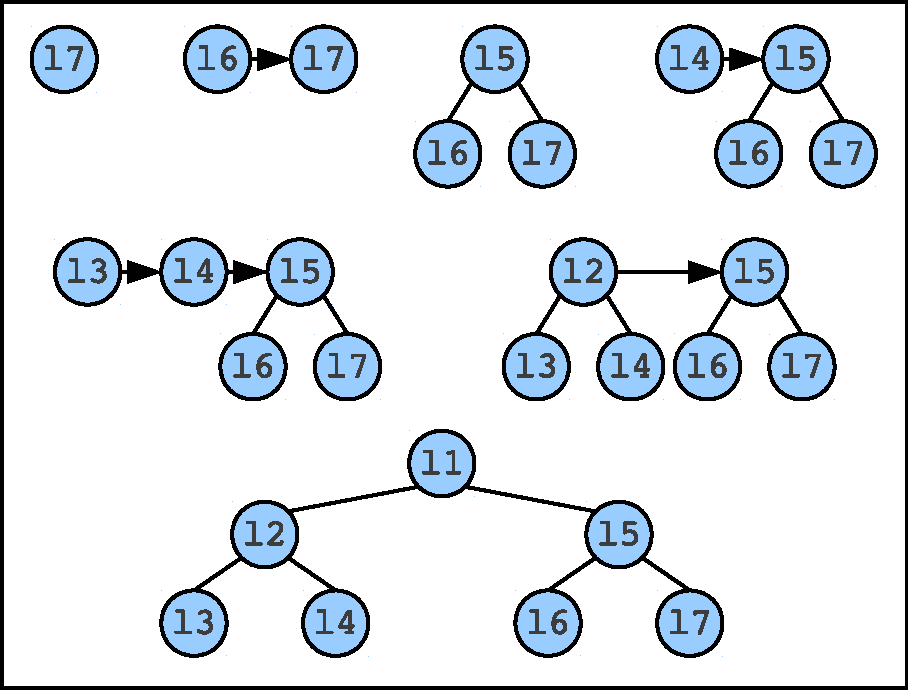
\includegraphics[scale=0.5]{insert.pdf}
\end{center}
\caption{Insertion in a Skew} \label{fig:insert}
\end{figure}

Insertion maintaining the invariant is constant time
and considers two cases: 
(1) when the spine has at least two trees
and the first two trees are of equal size,
we remove them and insert a new node built
of the new element and the two trees removed; and
(2) we just insert a new leaf.
In Figure~\ref{fig:insert} we show a graphic representation of
the successive skew lists that arise in the process of construction of a skew list with the elements of \ensuremath{\Varid{rList}} from section \ref{sec:extensiblerecords}.
Nodes connected by arrows represent linked-lists and nodes connected by lines represent trees.
The first two steps (adding elements with label \ensuremath{\Varid{l7}} and \ensuremath{\Varid{l6}}) are in case (2), 
thus two leaves are inserted into the spine. 
On the other hand, the third step (adding an element with label \ensuremath{\Varid{l5}}) is in case (1), so a node has to be built with the new element as root and the two previous trees as subtrees.

Skew lists are not optimal for merging records.  In the view of tree
instances as numbers, merging is equivalent to number addition.  Some
priority queue structures do support fast merging (or melding), but
usually the resulting trees are very deep and do not support efficient
access to some elements.

\subsection{SkewRecord}

In this subsection we present our implementation of extensible records
using (heterogeneous) skew lists. 
First, we introduce some types to model heterogeneous binary trees:

\begin{hscode}\SaveRestoreHook
\column{B}{@{}>{\hspre}l<{\hspost}@{}}%
\column{7}{@{}>{\hspre}l<{\hspost}@{}}%
\column{14}{@{}>{\hspre}l<{\hspost}@{}}%
\column{17}{@{}>{\hspre}l<{\hspost}@{}}%
\column{20}{@{}>{\hspre}l<{\hspost}@{}}%
\column{24}{@{}>{\hspre}c<{\hspost}@{}}%
\column{24E}{@{}l@{}}%
\column{27}{@{}>{\hspre}l<{\hspost}@{}}%
\column{34}{@{}>{\hspre}l<{\hspost}@{}}%
\column{37}{@{}>{\hspre}l<{\hspost}@{}}%
\column{40}{@{}>{\hspre}l<{\hspost}@{}}%
\column{E}{@{}>{\hspre}l<{\hspost}@{}}%
\>[B]{}\mathbf{data}\;{}\<[7]%
\>[7]{}\Conid{HEmpty}{}\<[24]%
\>[24]{}\mathrel{=}{}\<[24E]%
\>[27]{}\Conid{HEmpty}{}\<[E]%
\\
\>[B]{}\mathbf{data}\;{}\<[7]%
\>[7]{}\Conid{HNode}\;{}\<[14]%
\>[14]{}\Varid{e}\;{}\<[17]%
\>[17]{}\Varid{t}\;{}\<[20]%
\>[20]{}\Varid{t'}{}\<[24]%
\>[24]{}\mathrel{=}{}\<[24E]%
\>[27]{}\Conid{HNode}\;{}\<[34]%
\>[34]{}\Varid{e}\;{}\<[37]%
\>[37]{}\Varid{t}\;{}\<[40]%
\>[40]{}\Varid{t'}{}\<[E]%
\\
\>[B]{}\mathbf{type}\;{}\<[7]%
\>[7]{}\Conid{HLeaf}\;{}\<[14]%
\>[14]{}\Varid{e}{}\<[24]%
\>[24]{}\mathrel{=}{}\<[24E]%
\>[27]{}\Conid{HNode}\;\Varid{e}\;\Conid{HEmpty}\;\Conid{HEmpty}{}\<[E]%
\ColumnHook
\end{hscode}\resethooks
and a smart constructor for leaves:
\begin{hscode}\SaveRestoreHook
\column{B}{@{}>{\hspre}l<{\hspost}@{}}%
\column{14}{@{}>{\hspre}l<{\hspost}@{}}%
\column{24}{@{}>{\hspre}c<{\hspost}@{}}%
\column{24E}{@{}l@{}}%
\column{27}{@{}>{\hspre}l<{\hspost}@{}}%
\column{E}{@{}>{\hspre}l<{\hspost}@{}}%
\>[B]{}\Varid{hLeaf}\;{}\<[14]%
\>[14]{}\Varid{e}{}\<[24]%
\>[24]{}\mathrel{=}{}\<[24E]%
\>[27]{}\Conid{HNode}\;\Varid{e}\;\Conid{HEmpty}\;\Conid{HEmpty}{}\<[E]%
\ColumnHook
\end{hscode}\resethooks

\noindent
The element precedes the subtrees in \ensuremath{\Conid{HNode}}
so all elements in expressions read in order left to right.
The common leaf case warrants the helper type \ensuremath{\Conid{HLeaf}}
and the smart constructor \ensuremath{\Varid{hLeaf}}. 

A (heterogeneous) skew list is then defined as a heterogeneous list of (heterogeneous) binary trees. 
The following declarations define a skew list with the elements of the fourth step of Figure~\ref{fig:insert}:

\begin{hscode}\SaveRestoreHook
\column{B}{@{}>{\hspre}l<{\hspost}@{}}%
\column{5}{@{}>{\hspre}l<{\hspost}@{}}%
\column{12}{@{}>{\hspre}l<{\hspost}@{}}%
\column{20}{@{}>{\hspre}l<{\hspost}@{}}%
\column{25}{@{}>{\hspre}c<{\hspost}@{}}%
\column{25E}{@{}l@{}}%
\column{30}{@{}>{\hspre}l<{\hspost}@{}}%
\column{32}{@{}>{\hspre}c<{\hspost}@{}}%
\column{32E}{@{}l@{}}%
\column{37}{@{}>{\hspre}l<{\hspost}@{}}%
\column{E}{@{}>{\hspre}l<{\hspost}@{}}%
\>[B]{}\Varid{four}\mathrel{=}{}\<[E]%
\\
\>[B]{}\hsindent{5}{}\<[5]%
\>[5]{}\Conid{HCons}\;{}\<[12]%
\>[12]{}(\Varid{hLeaf}\;{}\<[20]%
\>[20]{}(\Conid{L4}{}\<[25]%
\>[25]{}\mathbin{.\!\!=\!\!.}{}\<[25E]%
\>[30]{}\text{\tt 'c'}))\mathbin{\$}{}\<[E]%
\\
\>[B]{}\hsindent{5}{}\<[5]%
\>[5]{}\Conid{HCons}\;{}\<[12]%
\>[12]{}(\Conid{HNode}\;{}\<[20]%
\>[20]{}(\Conid{L5}{}\<[25]%
\>[25]{}\mathbin{.\!\!=\!\!.}{}\<[25E]%
\>[30]{}\Conid{Nothing})\;{}\<[E]%
\\
\>[20]{}(\Varid{hLeaf}\;(\Conid{L6}{}\<[32]%
\>[32]{}\mathbin{.\!\!=\!\!.}{}\<[32E]%
\>[37]{}[\mskip1.5mu \mathrm{4},\mathrm{5}\mskip1.5mu]))\;{}\<[E]%
\\
\>[20]{}(\Varid{hLeaf}\;(\Conid{L7}{}\<[32]%
\>[32]{}\mathbin{.\!\!=\!\!.}{}\<[32E]%
\>[37]{}\text{\tt \char34 last\char34})))\mathbin{\$}{}\<[E]%
\\
\>[B]{}\hsindent{5}{}\<[5]%
\>[5]{}\Conid{HNil}{}\<[E]%
\ColumnHook
\end{hscode}\resethooks

%% $ fix emacs color highlighting

\subsubsection{Construction}

We define a smart constructor \ensuremath{\Varid{emptySkewRecord}} for empty skew lists, i.e. an empty list of trees.

\begin{hscode}\SaveRestoreHook
\column{B}{@{}>{\hspre}l<{\hspost}@{}}%
\column{E}{@{}>{\hspre}l<{\hspost}@{}}%
\>[B]{}\Varid{emptySkewRecord}\mathrel{=}\Conid{HNil}{}\<[E]%
\ColumnHook
\end{hscode}\resethooks

%\noindent
\ensuremath{\Conid{HHeight}} returns the height of a tree.
We will use it to detect the case of two leading equal height trees in the spine.
%
\begin{hscode}\SaveRestoreHook
\column{B}{@{}>{\hspre}l<{\hspost}@{}}%
\column{11}{@{}>{\hspre}l<{\hspost}@{}}%
\column{E}{@{}>{\hspre}l<{\hspost}@{}}%
\>[B]{}\mathbf{class}\;\Conid{HHeight}\;\Varid{t}\;\Varid{h}\mid \Varid{t}\to \Varid{h}{}\<[E]%
\\
\>[B]{}\mathbf{instance}\;{}\<[11]%
\>[11]{}\Conid{HHeight}\;\Conid{HEmpty}\;\Conid{HZero}{}\<[E]%
\\
\>[B]{}\mathbf{instance}\;{}\<[11]%
\>[11]{}\Conid{HHeight}\;\Varid{t}\;\Varid{h}\Rightarrow {}\<[E]%
\\
\>[11]{}\Conid{HHeight}\;(\Conid{HNode}\;\Varid{e}\;\Varid{t}\;\Varid{t'})\;(\Conid{HSucc}\;\Varid{h}){}\<[E]%
\ColumnHook
\end{hscode}\resethooks

\noindent
\ensuremath{\Conid{HSkewCarry}} finds out if a skew list \ensuremath{\Varid{l}} is in case (1) or (2). 
This will be used for insertion to decide whether we need to take the two leading existing trees
and put them below a new \ensuremath{\Conid{HNode}} (case 1),
or just insert a new \ensuremath{\Conid{HLeaf}} (case 2).
In the numerical representation of data structures,
adding an item is incrementing the number.
If each top level tree is a digit,
building a new taller tree is a form of carry,
so \ensuremath{\Conid{HSkewCarry}} returns \ensuremath{\Conid{HTrue}}.
%
\begin{hscode}\SaveRestoreHook
\column{B}{@{}>{\hspre}l<{\hspost}@{}}%
\column{E}{@{}>{\hspre}l<{\hspost}@{}}%
\>[B]{}\mathbf{class}\;\Conid{HSkewCarry}\;\Varid{l}\;\Varid{b}\mid \Varid{l}\to \Varid{b}{}\<[E]%
\\[\blanklineskip]%
\>[B]{}\Varid{hSkewCarry}\mathbin{::}\Conid{HSkewCarry}\;\Varid{l}\;\Varid{b}\Rightarrow \Varid{l}\to \Varid{b}{}\<[E]%
\\
\>[B]{}\Varid{hSkewCarry}\mathrel{=}\bot {}\<[E]%
\ColumnHook
\end{hscode}\resethooks
%
If the spine has none or one single tree we return \ensuremath{\Conid{HFalse}}.
\begin{hscode}\SaveRestoreHook
\column{B}{@{}>{\hspre}l<{\hspost}@{}}%
\column{E}{@{}>{\hspre}l<{\hspost}@{}}%
\>[B]{}\mathbf{instance}\;\Conid{HSkewCarry}\;\Conid{HNil}\;\Conid{HFalse}{}\<[E]%
\\
\>[B]{}\mathbf{instance}\;\Conid{HSkewCarry}\;(\Conid{HCons}\;\Varid{t}\;\Conid{HNil})\;\Conid{HFalse}{}\<[E]%
\ColumnHook
\end{hscode}\resethooks
%
In case the spine has more than one tree, 
we return \ensuremath{\Conid{HTrue}} if the first two trees are of equal size and
\ensuremath{\Conid{HFalse}} otherwise.
%
\begin{hscode}\SaveRestoreHook
\column{B}{@{}>{\hspre}l<{\hspost}@{}}%
\column{5}{@{}>{\hspre}c<{\hspost}@{}}%
\column{5E}{@{}l@{}}%
\column{8}{@{}>{\hspre}l<{\hspost}@{}}%
\column{E}{@{}>{\hspre}l<{\hspost}@{}}%
\>[B]{}\mathbf{instance}{}\<[E]%
\\
\>[B]{}\hsindent{5}{}\<[5]%
\>[5]{}({}\<[5E]%
\>[8]{}\Conid{HHeight}\;\Varid{t}\;\Varid{h}{}\<[E]%
\\
\>[B]{}\hsindent{5}{}\<[5]%
\>[5]{},{}\<[5E]%
\>[8]{}\Conid{HHeight}\;\Varid{t'}\;\Varid{h'}{}\<[E]%
\\
\>[B]{}\hsindent{5}{}\<[5]%
\>[5]{},{}\<[5E]%
\>[8]{}\Conid{HEq}\;\Varid{h}\;\Varid{h'}\;\Varid{b})\Rightarrow {}\<[E]%
\\
\>[8]{}\Conid{HSkewCarry}\;(\Conid{HCons}\;\Varid{t}\;(\Conid{HCons}\;\Varid{t'}\;\Varid{ts}))\;\Varid{b}{}\<[E]%
\ColumnHook
\end{hscode}\resethooks

All these pieces allow us to define \ensuremath{\Conid{HSkewExtend}},
which resembles the \ensuremath{\Conid{HCons}} constructor.
\begin{hscode}\SaveRestoreHook
\column{B}{@{}>{\hspre}l<{\hspost}@{}}%
\column{5}{@{}>{\hspre}l<{\hspost}@{}}%
\column{E}{@{}>{\hspre}l<{\hspost}@{}}%
\>[B]{}\mathbf{class}\;\Conid{HSkewExtend}\;\Varid{f}\;\Varid{r}\;\Varid{r'}\mid \Varid{f}\;\Varid{r}\to \Varid{r'}{}\<[E]%
\\
\>[B]{}\hsindent{5}{}\<[5]%
\>[5]{}\mathbf{where}\;\Varid{hSkewExtend}\mathbin{::}\Varid{f}\to \Varid{r}\to \Varid{r'}{}\<[E]%
\\
\>[B]{}\mathbf{infixr}\;\mathrm{2}\mathbin{`\Varid{hSkewExtend}`}{}\<[E]%
\ColumnHook
\end{hscode}\resethooks
\ensuremath{\Conid{HSkewExtend}} looks like \ensuremath{\Conid{HListGet}} shown earlier.
\ensuremath{\Conid{HSkewCarry}} is now responsible for discriminating
the current case,
while \ensuremath{\Conid{HListGet}} used \ensuremath{\Conid{HEq}} on the two labels.
%A smart test type-function saves on repetition.

\begin{hscode}\SaveRestoreHook
\column{B}{@{}>{\hspre}l<{\hspost}@{}}%
\column{5}{@{}>{\hspre}l<{\hspost}@{}}%
\column{8}{@{}>{\hspre}l<{\hspost}@{}}%
\column{9}{@{}>{\hspre}l<{\hspost}@{}}%
\column{24}{@{}>{\hspre}l<{\hspost}@{}}%
\column{E}{@{}>{\hspre}l<{\hspost}@{}}%
\>[B]{}\mathbf{instance}{}\<[E]%
\\
\>[B]{}\hsindent{5}{}\<[5]%
\>[5]{}({}\<[8]%
\>[8]{}\Conid{HSkewCarry}\;\Varid{r}\;\Varid{b}{}\<[E]%
\\
\>[B]{}\hsindent{5}{}\<[5]%
\>[5]{},{}\<[8]%
\>[8]{}\Conid{HSkewExtend'}\;\Varid{b}\;{}\<[24]%
\>[24]{}\Varid{f}\;\Varid{r}\;\Varid{r'})\Rightarrow {}\<[E]%
\\
\>[8]{}\Conid{HSkewExtend}\;{}\<[24]%
\>[24]{}\Varid{f}\;\Varid{r}\;\Varid{r'}\;\mathbf{where}{}\<[E]%
\\
\>[B]{}\hsindent{5}{}\<[5]%
\>[5]{}\Varid{hSkewExtend}\;\Varid{f}\;\Varid{r}\mathrel{=}{}\<[E]%
\\
\>[5]{}\hsindent{4}{}\<[9]%
\>[9]{}\Varid{hSkewExtend'}\;(\Varid{hSkewCarry}\;\Varid{r})\;\Varid{f}\;\Varid{r}{}\<[E]%
\\[\blanklineskip]%
\>[B]{}\mathbf{class}\;\Conid{HSkewExtend'}\;\Varid{b}\;\Varid{f}\;\Varid{r}\;\Varid{r'}\mid \Varid{b}\;\Varid{f}\;\Varid{r}\to \Varid{r'}\;\mathbf{where}{}\<[E]%
\\
\>[B]{}\hsindent{5}{}\<[5]%
\>[5]{}\Varid{hSkewExtend'}\mathbin{::}\Varid{b}\to \Varid{f}\to \Varid{r}\to \Varid{r'}{}\<[E]%
\ColumnHook
\end{hscode}\resethooks
\noindent
Here \ensuremath{\Conid{HFalse}} means that we should not add up the first two trees of the spine.
Either the size of the two leading trees are different, or the spine is empty or a singleton.
We just use \ensuremath{\Conid{HLeaf}} to insert a new tree at the beginning of the spine.
\begin{hscode}\SaveRestoreHook
\column{B}{@{}>{\hspre}l<{\hspost}@{}}%
\column{5}{@{}>{\hspre}l<{\hspost}@{}}%
\column{9}{@{}>{\hspre}l<{\hspost}@{}}%
\column{E}{@{}>{\hspre}l<{\hspost}@{}}%
\>[B]{}\mathbf{instance}{}\<[E]%
\\
\>[B]{}\hsindent{5}{}\<[5]%
\>[5]{}\Conid{HSkewExtend'}\;{}\<[E]%
\\
\>[5]{}\hsindent{4}{}\<[9]%
\>[9]{}\Conid{HFalse}\;{}\<[E]%
\\
\>[5]{}\hsindent{4}{}\<[9]%
\>[9]{}\Varid{f}\;{}\<[E]%
\\
\>[5]{}\hsindent{4}{}\<[9]%
\>[9]{}\Varid{r}\;{}\<[E]%
\\
\>[5]{}\hsindent{4}{}\<[9]%
\>[9]{}(\Conid{HCons}\;(\Conid{HLeaf}\;\Varid{f})\;\Varid{r})\;\mathbf{where}{}\<[E]%
\\
\>[B]{}\hsindent{5}{}\<[5]%
\>[5]{}\Varid{hSkewExtend'}\;\anonymous \;\Varid{f}\;\Varid{r}\mathrel{=}\Conid{HCons}\;(\Varid{hLeaf}\;\Varid{f})\;\Varid{r}{}\<[E]%
\ColumnHook
\end{hscode}\resethooks
%
When \ensuremath{\Conid{HSkewCarry}} returns \ensuremath{\Conid{HTrue}}, however, we build a new tree reusing the two trees that were at the start of the spine.
The length of the spine is reduced in one, since we take two elements but only add one.
%
\begin{hscode}\SaveRestoreHook
\column{B}{@{}>{\hspre}l<{\hspost}@{}}%
\column{5}{@{}>{\hspre}l<{\hspost}@{}}%
\column{9}{@{}>{\hspre}l<{\hspost}@{}}%
\column{E}{@{}>{\hspre}l<{\hspost}@{}}%
\>[B]{}\mathbf{instance}{}\<[E]%
\\
\>[B]{}\hsindent{5}{}\<[5]%
\>[5]{}\Conid{HSkewExtend'}\;{}\<[E]%
\\
\>[5]{}\hsindent{4}{}\<[9]%
\>[9]{}\Conid{HTrue}\;{}\<[E]%
\\
\>[5]{}\hsindent{4}{}\<[9]%
\>[9]{}\Varid{f}\;{}\<[E]%
\\
\>[5]{}\hsindent{4}{}\<[9]%
\>[9]{}(\Conid{HCons}\;\Varid{t}\;(\Conid{HCons}\;\Varid{t'}\;\Varid{r}))\;{}\<[E]%
\\
\>[5]{}\hsindent{4}{}\<[9]%
\>[9]{}(\Conid{HCons}\;(\Conid{HNode}\;\Varid{f}\;\Varid{t}\;\Varid{t'})\;\Varid{r})\;\mathbf{where}{}\<[E]%
\\
\>[B]{}\hsindent{5}{}\<[5]%
\>[5]{}\Varid{hSkewExtend'}\;\anonymous \;\Varid{f}\;(\Conid{HCons}\;\Varid{t}\;(\Conid{HCons}\;\Varid{t'}\;\Varid{r}))\mathrel{=}{}\<[E]%
\\
\>[5]{}\hsindent{4}{}\<[9]%
\>[9]{}(\Conid{HCons}\;(\Conid{HNode}\;\Varid{f}\;\Varid{t}\;\Varid{t'})\;\Varid{r}){}\<[E]%
\ColumnHook
\end{hscode}\resethooks

\subsubsection{Lookup}

%The missing piece is
Now, we turn to the introduction of \ensuremath{\Conid{HSkewGet}},
which explores all paths at compile time
but follows only the right one at run time.

\begin{hscode}\SaveRestoreHook
\column{B}{@{}>{\hspre}l<{\hspost}@{}}%
\column{5}{@{}>{\hspre}l<{\hspost}@{}}%
\column{E}{@{}>{\hspre}l<{\hspost}@{}}%
\>[B]{}\mathbf{class}\;\Conid{HSkewGet}\;\Varid{r}\;\Varid{l}\;\Varid{v}\mid \Varid{r}\;\Varid{l}\to \Varid{v}\;\mathbf{where}{}\<[E]%
\\
\>[B]{}\hsindent{5}{}\<[5]%
\>[5]{}\Varid{hSkewGet}\mathbin{::}\Varid{r}\to \Varid{l}\to \Varid{v}{}\<[E]%
\ColumnHook
\end{hscode}\resethooks
Deciding on the path to the desired field
is now more involved.
The cases that both the test function and the worker function must consider
are more numerous and long.
Thus, we merge both functions.
\ensuremath{\Conid{HSkewGet}} returns a type level and value level Maybe,
that is,
\ensuremath{\Conid{HNothing}} when no field with the label is found,
and \ensuremath{\Conid{HJust}} of the field's type/value otherwise.
For branching constructors \ensuremath{\Conid{HCons}} and \ensuremath{\Conid{HNode}},
\ensuremath{\Conid{HPlus}} (presented in subsection~\ref{sec:hlist}) chooses the correct path for us.

We will run \ensuremath{\Conid{HSkewGet}} on both the spine and each tree, so we have two base cases.
\ensuremath{\Conid{HNil}} is encountered at the end of the spine, and \ensuremath{\Conid{HEmpty}} at the bottom of trees.
In both cases, the field was not found, so we return \ensuremath{\Conid{HNothing}}.
\begin{hscode}\SaveRestoreHook
\column{B}{@{}>{\hspre}l<{\hspost}@{}}%
\column{5}{@{}>{\hspre}l<{\hspost}@{}}%
\column{E}{@{}>{\hspre}l<{\hspost}@{}}%
\>[B]{}\mathbf{instance}\;\Conid{HSkewGet}\;\Conid{HNil}\;\Varid{l}\;\Conid{HNothing}\;\mathbf{where}{}\<[E]%
\\
\>[B]{}\hsindent{5}{}\<[5]%
\>[5]{}\Varid{hSkewGet}\;\anonymous \;\anonymous \mathrel{=}\Conid{HNothing}{}\<[E]%
\\
\>[B]{}\mathbf{instance}\;\Conid{HSkewGet}\;\Conid{HEmpty}\;\Varid{l}\;\Conid{HNothing}\;\mathbf{where}{}\<[E]%
\\
\>[B]{}\hsindent{5}{}\<[5]%
\>[5]{}\Varid{hSkewGet}\;\anonymous \;\anonymous \mathrel{=}\Conid{HNothing}{}\<[E]%
\ColumnHook
\end{hscode}\resethooks
The \ensuremath{\Conid{HCons}} case must consider that the field may be found on the current tree or further down the spine.
A recursive call is made for each sub-case, and the results are combined with \ensuremath{\Conid{HPlus}}.
If the field is found in the current tree,
\ensuremath{\Conid{HPlus}} returns it, otherwise, it returns what the search down the spine did.
%
\begin{hscode}\SaveRestoreHook
\column{B}{@{}>{\hspre}l<{\hspost}@{}}%
\column{5}{@{}>{\hspre}l<{\hspost}@{}}%
\column{8}{@{}>{\hspre}l<{\hspost}@{}}%
\column{9}{@{}>{\hspre}l<{\hspost}@{}}%
\column{21}{@{}>{\hspre}l<{\hspost}@{}}%
\column{E}{@{}>{\hspre}l<{\hspost}@{}}%
\>[B]{}\mathbf{instance}{}\<[E]%
\\
\>[B]{}\hsindent{5}{}\<[5]%
\>[5]{}({}\<[8]%
\>[8]{}\Conid{HSkewGet}\;\Varid{r}\;{}\<[21]%
\>[21]{}\Varid{l}\;\Varid{vr}{}\<[E]%
\\
\>[B]{}\hsindent{5}{}\<[5]%
\>[5]{},{}\<[8]%
\>[8]{}\Conid{HSkewGet}\;\Varid{r'}\;{}\<[21]%
\>[21]{}\Varid{l}\;\Varid{vr'}{}\<[E]%
\\
\>[B]{}\hsindent{5}{}\<[5]%
\>[5]{},{}\<[8]%
\>[8]{}\Conid{HPlus}\;\Varid{vr}\;\Varid{vr'}\;\Varid{v})\Rightarrow {}\<[E]%
\\
\>[8]{}\Conid{HSkewGet}\;(\Conid{HCons}\;\Varid{r}\;\Varid{r'})\;\Varid{l}\;\Varid{v}\;\mathbf{where}{}\<[E]%
\\
\>[B]{}\hsindent{5}{}\<[5]%
\>[5]{}\Varid{hSkewGet}\;(\Conid{HCons}\;\Varid{r}\;\Varid{r'})\;\Varid{l}\mathrel{=}{}\<[E]%
\\
\>[5]{}\hsindent{4}{}\<[9]%
\>[9]{}\Varid{hSkewGet}\;\Varid{r}\;\Varid{l}\mathbin{`\Varid{hPlus}`}\Varid{hSkewGet}\;\Varid{r'}\;\Varid{l}{}\<[E]%
\ColumnHook
\end{hscode}\resethooks
%
Observe that when doing \ensuremath{\Varid{hSkewGet}\;\Varid{r}\;\Varid{l}\mathbin{`\Varid{hPlus}`}\Varid{hSkewGet}\;\Varid{r'}\;\Varid{l}} if the label is not present in \ensuremath{\Varid{r}} then 
the type system chooses the second instance of \ensuremath{\Conid{HPlus}}  (\ensuremath{\Conid{HPlus}\;\Conid{HNothing}\;\Varid{b}\;\Varid{b}}).
Thus, by lazy evaluation, the subexpression \ensuremath{\Varid{hSkewGet}\;\Varid{r}\;\Varid{l}} is not evaluated
since \ensuremath{\Varid{hPlus}} in that case simply returns its second argument.

\noindent The \ensuremath{\Conid{HNode}} case is a bigger version of the \ensuremath{\Conid{HCons}} case.
Here three recursive calls are made,
for the current field, the left tree, and the right tree.
Thus two \ensuremath{\Conid{HPlus}} calls are needed to combine the result.
%
\begin{hscode}\SaveRestoreHook
\column{B}{@{}>{\hspre}l<{\hspost}@{}}%
\column{5}{@{}>{\hspre}l<{\hspost}@{}}%
\column{8}{@{}>{\hspre}l<{\hspost}@{}}%
\column{9}{@{}>{\hspre}l<{\hspost}@{}}%
\column{13}{@{}>{\hspre}l<{\hspost}@{}}%
\column{16}{@{}>{\hspre}l<{\hspost}@{}}%
\column{19}{@{}>{\hspre}l<{\hspost}@{}}%
\column{21}{@{}>{\hspre}l<{\hspost}@{}}%
\column{24}{@{}>{\hspre}l<{\hspost}@{}}%
\column{26}{@{}>{\hspre}l<{\hspost}@{}}%
\column{E}{@{}>{\hspre}l<{\hspost}@{}}%
\>[B]{}\mathbf{instance}{}\<[E]%
\\
\>[B]{}\hsindent{5}{}\<[5]%
\>[5]{}({}\<[8]%
\>[8]{}\Conid{HSkewGet}\;\Varid{f}\;{}\<[21]%
\>[21]{}\Varid{l}\;\Varid{vf}{}\<[E]%
\\
\>[B]{}\hsindent{5}{}\<[5]%
\>[5]{},{}\<[8]%
\>[8]{}\Conid{HSkewGet}\;\Varid{r}\;{}\<[21]%
\>[21]{}\Varid{l}\;\Varid{vr}{}\<[E]%
\\
\>[B]{}\hsindent{5}{}\<[5]%
\>[5]{},{}\<[8]%
\>[8]{}\Conid{HSkewGet}\;\Varid{r'}\;{}\<[21]%
\>[21]{}\Varid{l}\;\Varid{vr'}{}\<[E]%
\\
\>[B]{}\hsindent{5}{}\<[5]%
\>[5]{},{}\<[8]%
\>[8]{}\Conid{HPlus}\;\Varid{vf}\;{}\<[19]%
\>[19]{}\Varid{vr}\;{}\<[26]%
\>[26]{}\Varid{vfr}{}\<[E]%
\\
\>[B]{}\hsindent{5}{}\<[5]%
\>[5]{},{}\<[8]%
\>[8]{}\Conid{HPlus}\;\Varid{vfr}\;{}\<[19]%
\>[19]{}\Varid{vr'}\;{}\<[24]%
\>[24]{}\Varid{v})\Rightarrow {}\<[E]%
\\
\>[8]{}\Conid{HSkewGet}\;(\Conid{HNode}\;\Varid{f}\;\Varid{r}\;\Varid{r'})\;\Varid{l}\;\Varid{v}\;\mathbf{where}{}\<[E]%
\\
\>[B]{}\hsindent{5}{}\<[5]%
\>[5]{}\Varid{hSkewGet}\;(\Conid{HNode}\;\Varid{f}\;\Varid{r}\;\Varid{r'})\;\Varid{l}\mathrel{=}{}\<[E]%
\\
\>[5]{}\hsindent{4}{}\<[9]%
\>[9]{}\Varid{hSkewGet}\;\Varid{f}\;\Varid{l}{}\<[E]%
\\
\>[9]{}\hsindent{4}{}\<[13]%
\>[13]{}\mathbin{`\Varid{hPlus}`}\Varid{hSkewGet}\;\Varid{r}\;\Varid{l}{}\<[E]%
\\
\>[13]{}\hsindent{3}{}\<[16]%
\>[16]{}\mathbin{`\Varid{hPlus}`}\Varid{hSkewGet}\;\Varid{r'}\;\Varid{l}{}\<[E]%
\ColumnHook
\end{hscode}\resethooks
%
Finally, the \ensuremath{\Conid{Field}} case, when a field is found, is the case 
%\alberto{cual, la que sigue o la anterior? no queda bien arrancar la orcion con And.....} 
that may actually build a \ensuremath{\Conid{HJust}} result.
As in \ensuremath{\Conid{HListGet}} for linked lists, \ensuremath{\Conid{HEq}} compares both labels.
We call \ensuremath{\Conid{HMakeMaybe}} with the result of the comparison,
and \ensuremath{\Conid{HNothing}} or \ensuremath{\Conid{HJust}} is returned as appropriate.
%
\begin{hscode}\SaveRestoreHook
\column{B}{@{}>{\hspre}l<{\hspost}@{}}%
\column{5}{@{}>{\hspre}l<{\hspost}@{}}%
\column{8}{@{}>{\hspre}l<{\hspost}@{}}%
\column{9}{@{}>{\hspre}l<{\hspost}@{}}%
\column{13}{@{}>{\hspre}l<{\hspost}@{}}%
\column{E}{@{}>{\hspre}l<{\hspost}@{}}%
\>[B]{}\mathbf{instance}{}\<[E]%
\\
\>[B]{}\hsindent{5}{}\<[5]%
\>[5]{}({}\<[8]%
\>[8]{}\Conid{HEq}\;\Varid{l}\;\Varid{l'}\;\Varid{b}{}\<[E]%
\\
\>[B]{}\hsindent{5}{}\<[5]%
\>[5]{},{}\<[8]%
\>[8]{}\Conid{HMakeMaybe}\;\Varid{b}\;\Varid{v}\;\Varid{m})\Rightarrow {}\<[E]%
\\
\>[8]{}\Conid{HSkewGet}\;(\Conid{Field}\;\Varid{l'}\;\Varid{v})\;\Varid{l}\;\Varid{m}\;\mathbf{where}{}\<[E]%
\\
\>[B]{}\hsindent{5}{}\<[5]%
\>[5]{}\Varid{hSkewGet}\;\Varid{f}\;\Varid{l}\mathrel{=}{}\<[E]%
\\
\>[5]{}\hsindent{4}{}\<[9]%
\>[9]{}\Varid{hMakeMaybe}\;{}\<[E]%
\\
\>[9]{}\hsindent{4}{}\<[13]%
\>[13]{}(\Varid{hEq}\;\Varid{l}\;(\Varid{label}\;\Varid{f}))\;{}\<[E]%
\\
\>[9]{}\hsindent{4}{}\<[13]%
\>[13]{}(\Varid{value}\;\Varid{f}){}\<[E]%
\ColumnHook
\end{hscode}\resethooks

When we repeat the experiment at the end of subsection \ref{sec:extensiblerecords}, 
but constructing a \ensuremath{\Conid{SkewRecord}} instead of an \ensuremath{\Conid{HList}}:
% using |emptySkewRecord| to construct a |SkewRecord|: \alberto{quien es |emptySkewRecord|?} 

%\alberto{yo capaz definiria un smart constructor que se llamara |hSkewEmpty| o por el estilo y lo pondria en lugar de HNil en la expresion de |rSkew|.}
%
\begin{hscode}\SaveRestoreHook
\column{B}{@{}>{\hspre}l<{\hspost}@{}}%
\column{3}{@{}>{\hspre}l<{\hspost}@{}}%
\column{8}{@{}>{\hspre}c<{\hspost}@{}}%
\column{8E}{@{}l@{}}%
\column{13}{@{}>{\hspre}l<{\hspost}@{}}%
\column{22}{@{}>{\hspre}c<{\hspost}@{}}%
\column{22E}{@{}l@{}}%
\column{25}{@{}>{\hspre}l<{\hspost}@{}}%
\column{E}{@{}>{\hspre}l<{\hspost}@{}}%
\>[B]{}\Varid{rSkew}\mathrel{=}{}\<[E]%
\\
\>[B]{}\hsindent{3}{}\<[3]%
\>[3]{}(\Conid{L1}{}\<[8]%
\>[8]{}\mathbin{.\!\!=\!\!.}{}\<[8E]%
\>[13]{}\Conid{True}{}\<[22]%
\>[22]{}){}\<[22E]%
\>[25]{}\mathbin{`\Varid{hSkewExtend}`}{}\<[E]%
\\
\>[B]{}\hsindent{3}{}\<[3]%
\>[3]{}(\Conid{L2}{}\<[8]%
\>[8]{}\mathbin{.\!\!=\!\!.}{}\<[8E]%
\>[13]{}\mathrm{9}{}\<[22]%
\>[22]{}){}\<[22E]%
\>[25]{}\mathbin{`\Varid{hSkewExtend}`}{}\<[E]%
\\
\>[B]{}\hsindent{3}{}\<[3]%
\>[3]{}(\Conid{L3}{}\<[8]%
\>[8]{}\mathbin{.\!\!=\!\!.}{}\<[8E]%
\>[13]{}\text{\tt \char34 bla\char34}{}\<[22]%
\>[22]{}){}\<[22E]%
\>[25]{}\mathbin{`\Varid{hSkewExtend}`}{}\<[E]%
\\
\>[B]{}\hsindent{3}{}\<[3]%
\>[3]{}(\Conid{L4}{}\<[8]%
\>[8]{}\mathbin{.\!\!=\!\!.}{}\<[8E]%
\>[13]{}\text{\tt 'c'}{}\<[22]%
\>[22]{}){}\<[22E]%
\>[25]{}\mathbin{`\Varid{hSkewExtend}`}{}\<[E]%
\\
\>[B]{}\hsindent{3}{}\<[3]%
\>[3]{}(\Conid{L5}{}\<[8]%
\>[8]{}\mathbin{.\!\!=\!\!.}{}\<[8E]%
\>[13]{}\Conid{Nothing}{}\<[22]%
\>[22]{}){}\<[22E]%
\>[25]{}\mathbin{`\Varid{hSkewExtend}`}{}\<[E]%
\\
\>[B]{}\hsindent{3}{}\<[3]%
\>[3]{}(\Conid{L6}{}\<[8]%
\>[8]{}\mathbin{.\!\!=\!\!.}{}\<[8E]%
\>[13]{}[\mskip1.5mu \mathrm{4},\mathrm{5}\mskip1.5mu]{}\<[22]%
\>[22]{}){}\<[22E]%
\>[25]{}\mathbin{`\Varid{hSkewExtend}`}{}\<[E]%
\\
\>[B]{}\hsindent{3}{}\<[3]%
\>[3]{}(\Conid{L7}{}\<[8]%
\>[8]{}\mathbin{.\!\!=\!\!.}{}\<[8E]%
\>[13]{}\text{\tt \char34 last\char34}{}\<[22]%
\>[22]{}){}\<[22E]%
\>[25]{}\mathbin{`\Varid{hSkewExtend}`}{}\<[E]%
\\
\>[B]{}\hsindent{3}{}\<[3]%
\>[3]{}\Varid{emptySkewRecord}{}\<[E]%
\\[\blanklineskip]%
\>[B]{}\Varid{lastSkew}\mathrel{=}\Varid{hSkewGet}\;\Varid{rSkew}\;\Conid{L7}{}\<[E]%
\ColumnHook
\end{hscode}\resethooks
the resulting core code is:

\begin{hscode}\SaveRestoreHook
\column{B}{@{}>{\hspre}l<{\hspost}@{}}%
\column{3}{@{}>{\hspre}l<{\hspost}@{}}%
\column{5}{@{}>{\hspre}l<{\hspost}@{}}%
\column{7}{@{}>{\hspre}l<{\hspost}@{}}%
\column{9}{@{}>{\hspre}l<{\hspost}@{}}%
\column{E}{@{}>{\hspre}l<{\hspost}@{}}%
\>[B]{}\Varid{lastSkewCore}\mathrel{=}\mathbf{case}\;\Varid{rSkew}\;\mathbf{of}{}\<[E]%
\\
\>[B]{}\hsindent{3}{}\<[3]%
\>[3]{}\Conid{HCons}\;\Varid{t1}\;\anonymous \to \mathbf{case}\;\Varid{t1}\;\mathbf{of}{}\<[E]%
\\
\>[3]{}\hsindent{2}{}\<[5]%
\>[5]{}\Conid{HNode}\;\anonymous \;\anonymous \;\Varid{t12}\to \mathbf{case}\;\Varid{t12}\;\mathbf{of}{}\<[E]%
\\
\>[5]{}\hsindent{2}{}\<[7]%
\>[7]{}\Conid{HNode}\;\anonymous \;\anonymous \;\Varid{t121}\to \mathbf{case}\;\Varid{t121}\;\mathbf{of}{}\<[E]%
\\
\>[7]{}\hsindent{2}{}\<[9]%
\>[9]{}\Conid{HNode}\;\Varid{e}\;\anonymous \;\anonymous \to \Varid{e}{}\<[E]%
\ColumnHook
\end{hscode}\resethooks
Thus, getting to \ensuremath{\Varid{l7}} at run time only traverses a (logarithmic length) fraction of the elements,
as we have seen in Figure~\ref{fig:search-skew}.
Later we will examine runtime benchmarks.


%%%%%%%%%%%%%%%%%%%%%%%%%%%%%%%%%%%%%%%%%%%%%%%%%%%%%%%%%%%%%%%%%%%%%%%%%%%%%%%%%%%%%%%%%%%%%%%%%%%%%%%%%%%%%%%%%%%%%

\subsubsection{Update}\label{sec:update}

%a type-function |HSkewUpdate| 
We now define an update operation that makes it possible to change
a field of some label with a new field with possibly new label and value.
%
\begin{hscode}\SaveRestoreHook
\column{B}{@{}>{\hspre}l<{\hspost}@{}}%
\column{5}{@{}>{\hspre}l<{\hspost}@{}}%
\column{E}{@{}>{\hspre}l<{\hspost}@{}}%
\>[B]{}\mathbf{class}\;\Conid{HSkewUpdate}\;\Varid{l}\;\Varid{e}\;\Varid{r}\;\Varid{r'}\mid \Varid{l}\;\Varid{e}\;\Varid{r}\to \Varid{r'}\;\mathbf{where}{}\<[E]%
\\
\>[B]{}\hsindent{5}{}\<[5]%
\>[5]{}\Varid{hSkewUpdate}\mathbin{::}\Varid{l}\to \Varid{e}\to \Varid{r}\to \Varid{r'}{}\<[E]%
\ColumnHook
\end{hscode}\resethooks
%
We use the lookup operation \ensuremath{\Conid{HSkewGet}} to discriminate at type-level
whether the field with the searched label is present or not in the skew list.
%
\begin{hscode}\SaveRestoreHook
\column{B}{@{}>{\hspre}l<{\hspost}@{}}%
\column{5}{@{}>{\hspre}l<{\hspost}@{}}%
\column{8}{@{}>{\hspre}l<{\hspost}@{}}%
\column{11}{@{}>{\hspre}l<{\hspost}@{}}%
\column{14}{@{}>{\hspre}l<{\hspost}@{}}%
\column{33}{@{}>{\hspre}l<{\hspost}@{}}%
\column{E}{@{}>{\hspre}l<{\hspost}@{}}%
\>[B]{}\mathbf{instance}\;{}\<[11]%
\>[11]{}({}\<[14]%
\>[14]{}\Conid{HSkewGet}\;\Varid{r}\;\Varid{l}\;\Varid{m}{}\<[E]%
\\
\>[11]{},{}\<[14]%
\>[14]{}\Conid{HSkewUpdate'}\;\Varid{m}\;\Varid{l}\;\Varid{e}\;\Varid{r}\;\Varid{r'})\Rightarrow {}\<[E]%
\\
\>[11]{}\Conid{HSkewUpdate}\;\Varid{l}\;\Varid{e}\;\Varid{r}\;\Varid{r'}\;{}\<[33]%
\>[33]{}\mathbf{where}{}\<[E]%
\\
\>[B]{}\hsindent{5}{}\<[5]%
\>[5]{}\Varid{hSkewUpdate}\;\Varid{l}\;\Varid{e}\;\Varid{r}\mathrel{=}{}\<[E]%
\\
\>[5]{}\hsindent{3}{}\<[8]%
\>[8]{}\Varid{hSkewUpdate'}\;(\Varid{hSkewGet}\;\Varid{r}\;\Varid{l})\;\Varid{l}\;\Varid{e}\;\Varid{r}{}\<[E]%
\\
\>[B]{}\;{}\<[E]%
\\
\>[B]{}\mathbf{class}\;\Conid{HSkewUpdate'}\;\Varid{m}\;\Varid{l}\;\Varid{e}\;\Varid{r}\;\Varid{r'}\mid \Varid{m}\;\Varid{l}\;\Varid{e}\;\Varid{r}\to \Varid{r'}\;\mathbf{where}{}\<[E]%
\\
\>[B]{}\hsindent{5}{}\<[5]%
\>[5]{}\Varid{hSkewUpdate'}\mathbin{::}\Varid{m}\to \Varid{l}\to \Varid{e}\to \Varid{r}\to \Varid{r'}{}\<[E]%
\ColumnHook
\end{hscode}\resethooks
%
In case the label is not present we have nothing to do than just returning the 
structure unchanged. 
%
\begin{hscode}\SaveRestoreHook
\column{B}{@{}>{\hspre}l<{\hspost}@{}}%
\column{5}{@{}>{\hspre}l<{\hspost}@{}}%
\column{41}{@{}>{\hspre}l<{\hspost}@{}}%
\column{E}{@{}>{\hspre}l<{\hspost}@{}}%
\>[B]{}\mathbf{instance}\;\Conid{HSkewUpdate'}\;\Conid{HNothing}\;\Varid{l}\;\Varid{e}\;\Varid{r}\;\Varid{r}\;{}\<[41]%
\>[41]{}\mathbf{where}{}\<[E]%
\\
\>[B]{}\hsindent{5}{}\<[5]%
\>[5]{}\Varid{hSkewUpdate'}\;\anonymous \;\Varid{l}\;\Varid{e}\;\Varid{r}\mathrel{=}\Varid{r}{}\<[E]%
\ColumnHook
\end{hscode}\resethooks
%
In the other cases (i.e. when lookup results in \ensuremath{\Conid{HJust}\;\Varid{v}}) we call \ensuremath{\Varid{hSkewUpdate}} recursively on all subparts in order to apply the update when necessary.
Because of the previous instance (when lookup returns \ensuremath{\Conid{HNothing}}), at run time recursion will not enter in those cases where the label is not present.
We start the process in the spine. 
%
\begin{hscode}\SaveRestoreHook
\column{B}{@{}>{\hspre}l<{\hspost}@{}}%
\column{5}{@{}>{\hspre}l<{\hspost}@{}}%
\column{8}{@{}>{\hspre}l<{\hspost}@{}}%
\column{9}{@{}>{\hspre}l<{\hspost}@{}}%
\column{16}{@{}>{\hspre}l<{\hspost}@{}}%
\column{33}{@{}>{\hspre}l<{\hspost}@{}}%
\column{E}{@{}>{\hspre}l<{\hspost}@{}}%
\>[B]{}\mathbf{instance}{}\<[E]%
\\
\>[B]{}\hsindent{5}{}\<[5]%
\>[5]{}({}\<[8]%
\>[8]{}\Conid{HSkewUpdate}\;\Varid{l}\;\Varid{e}\;\Varid{t}\;\Varid{t'}{}\<[E]%
\\
\>[B]{}\hsindent{5}{}\<[5]%
\>[5]{},{}\<[8]%
\>[8]{}\Conid{HSkewUpdate}\;\Varid{l}\;\Varid{e}\;\Varid{ts}\;\Varid{ts'})\Rightarrow {}\<[E]%
\\
\>[B]{}\hsindent{5}{}\<[5]%
\>[5]{}\Conid{HSkewUpdate'}\;(\Conid{HJust}\;\Varid{v})\;\Varid{l}\;\Varid{e}\;{}\<[33]%
\>[33]{}(\Conid{HCons}\;\Varid{t}\;\Varid{ts})\;{}\<[E]%
\\
\>[33]{}(\Conid{HCons}\;\Varid{t'}\;\Varid{ts'}){}\<[E]%
\\
\>[B]{}\hsindent{5}{}\<[5]%
\>[5]{}\mathbf{where}{}\<[E]%
\\
\>[B]{}\hsindent{5}{}\<[5]%
\>[5]{}\Varid{hSkewUpdate'}\;\anonymous \;\Varid{l}\;\Varid{e}\;(\Conid{HCons}\;\Varid{t}\;\Varid{ts})\mathrel{=}{}\<[E]%
\\
\>[5]{}\hsindent{4}{}\<[9]%
\>[9]{}\Conid{HCons}\;{}\<[16]%
\>[16]{}(\Varid{hSkewUpdate}\;\Varid{l}\;\Varid{e}\;\Varid{t})\;{}\<[E]%
\\
\>[16]{}(\Varid{hSkewUpdate}\;\Varid{l}\;\Varid{e}\;\Varid{ts}){}\<[E]%
\ColumnHook
\end{hscode}\resethooks
%
On a \ensuremath{\Conid{HNode}}, \ensuremath{\Varid{hSkewUpdate}} is recursively called on
the left and right sub-trees as well as on the element of the node.
\begin{hscode}\SaveRestoreHook
\column{B}{@{}>{\hspre}l<{\hspost}@{}}%
\column{5}{@{}>{\hspre}l<{\hspost}@{}}%
\column{8}{@{}>{\hspre}l<{\hspost}@{}}%
\column{9}{@{}>{\hspre}l<{\hspost}@{}}%
\column{16}{@{}>{\hspre}l<{\hspost}@{}}%
\column{33}{@{}>{\hspre}l<{\hspost}@{}}%
\column{E}{@{}>{\hspre}l<{\hspost}@{}}%
\>[B]{}\mathbf{instance}{}\<[E]%
\\
\>[B]{}\hsindent{5}{}\<[5]%
\>[5]{}({}\<[8]%
\>[8]{}\Conid{HSkewUpdate}\;\Varid{l}\;\Varid{e}\;\Varid{e'}\;\Varid{e''}{}\<[E]%
\\
\>[B]{}\hsindent{5}{}\<[5]%
\>[5]{},{}\<[8]%
\>[8]{}\Conid{HSkewUpdate}\;\Varid{l}\;\Varid{e}\;\Varid{tl}\;\Varid{tl'}{}\<[E]%
\\
\>[B]{}\hsindent{5}{}\<[5]%
\>[5]{},{}\<[8]%
\>[8]{}\Conid{HSkewUpdate}\;\Varid{l}\;\Varid{e}\;\Varid{tr}\;\Varid{tr'})\Rightarrow {}\<[E]%
\\
\>[B]{}\hsindent{5}{}\<[5]%
\>[5]{}\Conid{HSkewUpdate'}\;(\Conid{HJust}\;\Varid{v})\;\Varid{l}\;\Varid{e}\;{}\<[33]%
\>[33]{}(\Conid{HNode}\;\Varid{e'}\;\Varid{tl}\;\Varid{tr})\;{}\<[E]%
\\
\>[33]{}(\Conid{HNode}\;\Varid{e''}\;\Varid{tl'}\;\Varid{tr'}){}\<[E]%
\\
\>[B]{}\hsindent{5}{}\<[5]%
\>[5]{}\mathbf{where}{}\<[E]%
\\
\>[B]{}\hsindent{5}{}\<[5]%
\>[5]{}\Varid{hSkewUpdate'}\;\anonymous \;\Varid{l}\;\Varid{e}\;(\Conid{HNode}\;\Varid{e'}\;\Varid{tl}\;\Varid{tr})\mathrel{=}{}\<[E]%
\\
\>[5]{}\hsindent{4}{}\<[9]%
\>[9]{}\Conid{HNode}\;{}\<[16]%
\>[16]{}(\Varid{hSkewUpdate}\;\Varid{l}\;\Varid{e}\;\Varid{e'})\;{}\<[E]%
\\
\>[16]{}(\Varid{hSkewUpdate}\;\Varid{l}\;\Varid{e}\;\Varid{tl})\;{}\<[E]%
\\
\>[16]{}(\Varid{hSkewUpdate}\;\Varid{l}\;\Varid{e}\;\Varid{tr}){}\<[E]%
\ColumnHook
\end{hscode}\resethooks
%
Finally, when we arrive to a \ensuremath{\Conid{Field}} and we know the label is the one we
are searching for (because we are considering the case \ensuremath{\Conid{HJust}\;\Varid{v}}), we simply return the updated field. 
%
\begin{hscode}\SaveRestoreHook
\column{B}{@{}>{\hspre}l<{\hspost}@{}}%
\column{5}{@{}>{\hspre}l<{\hspost}@{}}%
\column{6}{@{}>{\hspre}l<{\hspost}@{}}%
\column{8}{@{}>{\hspre}l<{\hspost}@{}}%
\column{E}{@{}>{\hspre}l<{\hspost}@{}}%
\>[B]{}\mathbf{instance}{}\<[E]%
\\
\>[B]{}\hsindent{5}{}\<[5]%
\>[5]{}\Conid{HSkewUpdate'}\;(\Conid{HJust}\;\Varid{v})\;\Varid{l}\;\Varid{e}\;(\Conid{Field}\;\Varid{l}\;\Varid{v})\;\Varid{e}{}\<[E]%
\\
\>[5]{}\hsindent{1}{}\<[6]%
\>[6]{}\mathbf{where}{}\<[E]%
\\
\>[6]{}\hsindent{2}{}\<[8]%
\>[8]{}\Varid{hSkewUpdate'}\;\anonymous \;\Varid{l}\;\Varid{e}\;\Varid{e'}\mathrel{=}\Varid{e}{}\<[E]%
\ColumnHook
\end{hscode}\resethooks

At run time, this implementation of \ensuremath{\Varid{hSkewUpdate}} only
rebuilds the path to the field to update,
keeping all other sub-trees intact.
% Due to lazy evaluation, the searches of the label are performed only at compile time.
Thus the operation runs in time logarithmic in the size of the record.

\subsubsection{Remove}

Removing a field is easy based on updating.
We overwrite the field we want to eliminate with the first field in the skew list,
and then we remove the first field from the list.
Thus, we remove elements in logarithmic time while keeping the tree balanced.

First, we need a helper to remove the first element of a skew list.
%
\begin{hscode}\SaveRestoreHook
\column{B}{@{}>{\hspre}l<{\hspost}@{}}%
\column{5}{@{}>{\hspre}l<{\hspost}@{}}%
\column{E}{@{}>{\hspre}l<{\hspost}@{}}%
\>[B]{}\mathbf{class}\;\Conid{HSkewTail}\;\Varid{ts}\;\Varid{ts'}\mid \Varid{ts}\to \Varid{ts'}\;\mathbf{where}{}\<[E]%
\\
\>[B]{}\hsindent{5}{}\<[5]%
\>[5]{}\Varid{hSkewTail}\mathbin{::}\Varid{ts}\to \Varid{ts'}{}\<[E]%
\ColumnHook
\end{hscode}\resethooks

\noindent
In Figure~\ref{fig:tail} we show an example of the possible cases 
we can find.

\begin{figure}[htp]
\begin{center}
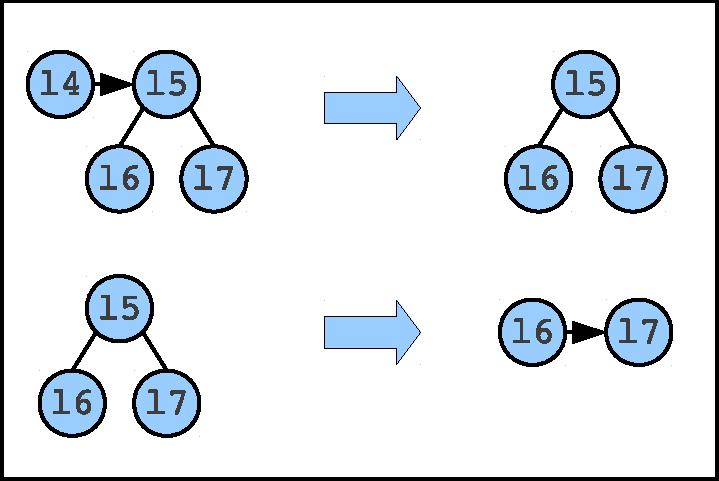
\includegraphics[scale=0.5]{tail.pdf}
\end{center}
\caption{Tail in a Skew} \label{fig:tail}
\end{figure}

The easy case is when the spine begins with a leaf.
We just return the tail of the spine list.
\begin{hscode}\SaveRestoreHook
\column{B}{@{}>{\hspre}l<{\hspost}@{}}%
\column{5}{@{}>{\hspre}l<{\hspost}@{}}%
\column{E}{@{}>{\hspre}l<{\hspost}@{}}%
\>[B]{}\mathbf{instance}\;\Conid{HSkewTail}\;(\Conid{HCons}\;(\Conid{HLeaf}\;\Varid{e})\;\Varid{ts})\;\Varid{ts}\;\mathbf{where}{}\<[E]%
\\
\>[B]{}\hsindent{5}{}\<[5]%
\>[5]{}\Varid{hSkewTail}\;(\Conid{HCons}\;\anonymous \;\Varid{ts})\mathrel{=}\Varid{ts}{}\<[E]%
\ColumnHook
\end{hscode}\resethooks

\noindent
The other case is when the spine begins with a tree of three or more elements.
Since \ensuremath{\Conid{HLeaf}} is a synonym of \ensuremath{\Conid{HNode}} with \ensuremath{\Conid{HEmpty}} as sub-trees,
we need to assert the case when the sub-trees of the root \ensuremath{\Conid{HNode}}
are nonempty (i.e. \ensuremath{\Conid{HNode}}s themselves).
By construction, both sub-trees have the same shape, but doing pattern matching on the first one only suffices to make sure this case does not overlap with the previous one.
In this case we grow the spine with the sub-trees, throwing away the root.
%
\begin{hscode}\SaveRestoreHook
\column{B}{@{}>{\hspre}l<{\hspost}@{}}%
\column{5}{@{}>{\hspre}l<{\hspost}@{}}%
\column{9}{@{}>{\hspre}l<{\hspost}@{}}%
\column{E}{@{}>{\hspre}l<{\hspost}@{}}%
\>[B]{}\mathbf{instance}{}\<[E]%
\\
\>[B]{}\hsindent{5}{}\<[5]%
\>[5]{}\Conid{HSkewTail}\;{}\<[E]%
\\
\>[5]{}\hsindent{4}{}\<[9]%
\>[9]{}(\Conid{HCons}\;(\Conid{HNode}\;\Varid{e}\;\Varid{t}\;(\Conid{HNode}\;\Varid{e'}\;\Varid{t'}\;\Varid{t''}))\;\Varid{ts})\;{}\<[E]%
\\
\>[5]{}\hsindent{4}{}\<[9]%
\>[9]{}(\Conid{HCons}\;\Varid{t}\;((\Conid{HCons}\;(\Conid{HNode}\;\Varid{e'}\;\Varid{t'}\;\Varid{t''}))\;\Varid{ts})){}\<[E]%
\\
\>[B]{}\hsindent{5}{}\<[5]%
\>[5]{}\mathbf{where}{}\<[E]%
\\
\>[B]{}\hsindent{5}{}\<[5]%
\>[5]{}\Varid{hSkewTail}\;(\Conid{HCons}\;(\Conid{HNode}\;\anonymous \;\Varid{t}\;\Varid{t'})\;\Varid{ts})\mathrel{=}{}\<[E]%
\\
\>[5]{}\hsindent{4}{}\<[9]%
\>[9]{}\Conid{HCons}\;\Varid{t}\;(\Conid{HCons}\;\Varid{t'}\;\Varid{ts}){}\<[E]%
\ColumnHook
\end{hscode}\resethooks


Last, \ensuremath{\Varid{hSkewRemove}} takes the first node and calls \ensuremath{\Varid{hSkewUpdate}}
to duplicate it where the label we want gone was.
Then \ensuremath{\Varid{hSkewTail}} removes the original occurrence,
at the start of the list.
\begin{hscode}\SaveRestoreHook
\column{B}{@{}>{\hspre}l<{\hspost}@{}}%
\column{9}{@{}>{\hspre}l<{\hspost}@{}}%
\column{E}{@{}>{\hspre}l<{\hspost}@{}}%
\>[B]{}\Varid{hSkewRemove}\;\Varid{l}\;(\Conid{HCons}\;(\Conid{HNode}\;\Varid{e}\;\Varid{t}\;\Varid{t'})\;\Varid{ts})\mathrel{=}{}\<[E]%
\\
\>[B]{}\hsindent{9}{}\<[9]%
\>[9]{}\Varid{hSkewTail}\mathbin{\$}{}\<[E]%
\\
\>[B]{}\hsindent{9}{}\<[9]%
\>[9]{}\Varid{hSkewUpdate}\;\Varid{l}\;\Varid{e}\;(\Conid{HCons}\;(\Conid{HNode}\;\Varid{e}\;\Varid{t}\;\Varid{t'})\;\Varid{ts}){}\<[E]%
\ColumnHook
\end{hscode}\resethooks

%% $ fix emacs color highlighting

%%%%%%%%%%%%%%%%%%%%%%%%%%%%%%%%%%%%%%%%%%%%%%%%%%%%%%%%%%%%%%%%%%%%%%%%%%%%%%%%%%%%%%%%%%%%%%%%%%%%%%%%%%%%%%%%%%%%%

\section{Efficiency}\label{sec:efficiency}

In order to chose the best implementation in practice and as a sanity check,
we did some synthetic benchmarks of the code.
We compile and run the programs in a 4 core 2.2 Ghz second genertion (Sandy Bridge) Intel i7 MacBook Pro Notebook with 8 GB of RAM.
We use GHC version 7.6.1 64 bits under OS X 10.8 Mountain Lion.

We time accessing the last of an increasing number of fields.
The program constructs the list once
and runs a 10 million iteration lookup loop,
taking the necessary precautions to avoid the compiler
exploiting the language lazyness to optimize out all our code.
Run time comparisons are shown in Figure~\ref{run_time}.

\begin{figure}[b]
\begin{center}
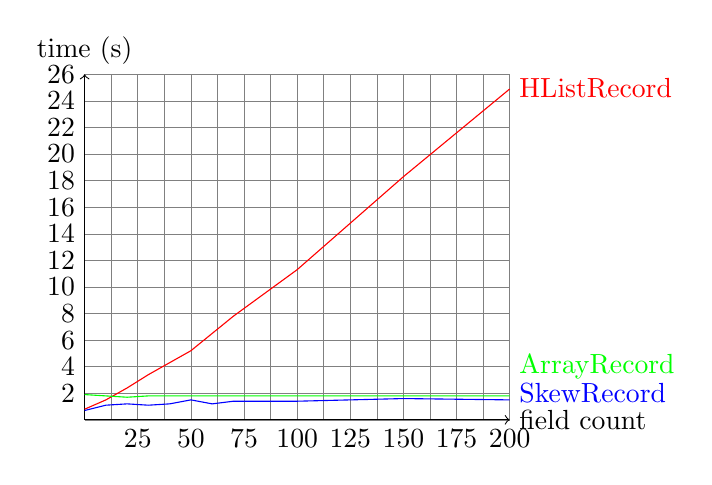
\begin{tikzpicture}[x=0.027cm,y=0.16875cm]

  \def\xmin{0}
  \def\xmax{200}
  \def\ymin{0}
  \def\ymax{26}

  % grid
  \draw[style=help lines, xstep=12.5, ystep=2] (\xmin,\ymin) grid
  (\xmax,\ymax);

  % axes
  \draw[->] (\xmin,\ymin) -- (\xmax,\ymin) node[right] {field count};
  \draw[->] (\xmin,\ymin) -- (\xmin,\ymax) node[above] {time (s)};

  % xticks and yticks
  \foreach \x in {25,50,...,\xmax}
  \node at (\x, \ymin) [below] {\x};
  \foreach \y in {2,4,...,\ymax}
  \node at (\xmin,\y) [left] {\y};

  \draw[red] plot coordinates {
    (0,  0.8)
    (10, 1.5)
    (20, 2.4)
    (30, 3.4)
    (40, 4.3)
    (50, 5.2)
    (60, 6.5)
    (70, 7.8)
    (100,11.3)
    (150,18.3)
    (200,24.9)
  };
  \node[right,red] at (200, 25) {HListRecord};


  \draw[green] plot coordinates {
    (0,  1.9)
    (10, 1.8)
    (20, 1.7)
    (30, 1.8)
    (40, 1.8)
    (50, 1.8)
    (60, 1.8)
    (70, 1.8)
    (100,1.8)
    (150,1.8)
    (200,1.8)
  };
  \node[right,green] at (200, 4) {ArrayRecord};

  \draw[blue] plot coordinates {
    (0,  0.7)
    (10, 1.1)
    (20, 1.2)
    (30, 1.1)
    (40, 1.2)
    (50, 1.5)
    (60, 1.2)
    (70, 1.4)
    (100,1.4)
    (150,1.6)
    (200,1.5)
  };
  \node[right,blue] at (200, 2) {SkewRecord};

\end{tikzpicture}
\end{center}
\caption{Lookup: run time}
\label{run_time}
\end{figure}

Note how in practice \ensuremath{\Conid{ArrayRecord}} and \ensuremath{\Conid{SkewRecord}} take the same time no matter the length of the record.
Actually, sometimes larger records run faster than smaller records for \ensuremath{\Conid{SkewRecord}}.
For example, a 31 size skew list contains a single tree,
so elements are at most 5 hops away.
But a 28 size skew lists contains trees sized
1, 1, 3, 7 and 15,
and getting to the last takes 8 hops.

Up to ten elements, simple linked lists are faster than skew lists.
By fusing the spine list and the tree nodes,
skew lists can be tweaked to improve the performance with few elements.
This results in a single node type,
with an element and three child node references,
one to the next node,
one to the right subtree,
and one to the node of the next tree.
We chose the unfused exposition for clarity.
Another option is to use linked list for small records and switch to
skew list when over 10 fields.
Since the test is done at compile time, the adaptive structure has no
run time overhead
above having to copy the 10 fields from the linked list to the tree
when the limit is surpassed.

\begin{figure}[t]
\begin{center}
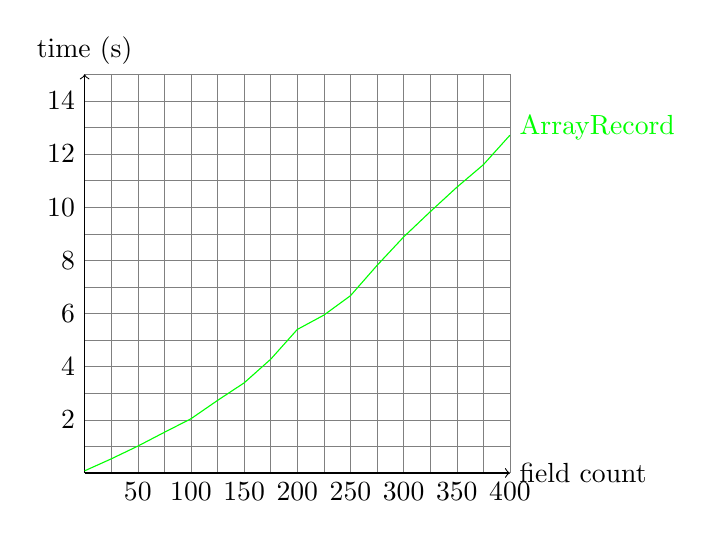
\begin{tikzpicture}[x=0.0135cm,y=0.3375cm]

  \def\xmin{0}
  \def\xmax{400}
  \def\ymin{0}
  \def\ymax{15}

  % grid
  \draw[style=help lines, xstep=25, ystep=1] (\xmin,\ymin) grid
  (\xmax,\ymax);

  % axes
  \draw[->] (\xmin,\ymin) -- (\xmax,\ymin) node[right] {field count};
  \draw[->] (\xmin,\ymin) -- (\xmin,\ymax) node[above] {time (s)};

  % xticks and yticks
  \foreach \x in {50,100,...,\xmax}
  \node at (\x, \ymin) [below] {\x};
  \foreach \y in {2,4,...,\ymax}
  \node at (\xmin,\y) [left] {\y};

  \draw[green] plot coordinates {
    (0,   0.08)
    (25,  0.53)
    (50,  1.01)
    (75,  1.53)
    (100, 2.04)
    (125, 2.73)
    (150, 3.39)
    (175, 4.28)
    (200, 5.40)
    (225, 5.94)
    (250, 6.67)
    (275, 7.81)
    (300, 8.88)
    (325, 9.83)
    (350,10.75)
    (375,11.60)
    (400,12.71)
  };
  \node[right,green] at (400, 13) {ArrayRecord};

\end{tikzpicture}
\end{center}
\caption{Extend: run time}
\label{extend_time}
\end{figure}


Next, Figure~\ref{extend_time} shows the runtime of inserting one more
field to a record of a given length.
To force the worst case for \ensuremath{\Conid{ArrayRecord}}, we disable the insertion optimization by immediately looking up the field just inserted.
The insert-lookup process is run one million times.
Only \ensuremath{\Conid{ArrayRecord}} is graphed because the other alternatives are too fast in this case.
The graph exposes the linear time behavior of \ensuremath{\Conid{ArrayRecord}}, its Achilles' heel.
However, we do not expect real life applications to fall in this case.
In general, multiple adjacent insertions preceding a lookup would be the common case. 

\begin{figure}[b]
\begin{center}
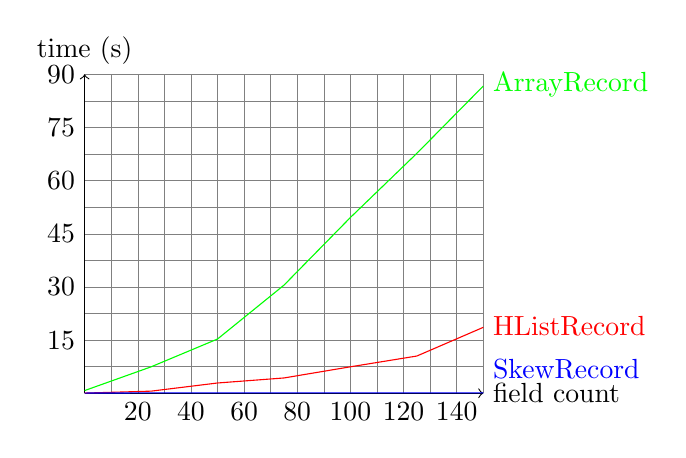
\begin{tikzpicture}[x=0.03375cm,y=0.045cm]

  \def\xmin{0}
  \def\xmax{150}
  \def\ymin{0}
  \def\ymax{90}

  % grid
  \draw[style=help lines, xstep=10, ystep=7.5] (\xmin,\ymin) grid
  (\xmax,\ymax);

  % axes
  \draw[->] (\xmin,\ymin) -- (\xmax,\ymin) node[right] {field count};
  \draw[->] (\xmin,\ymin) -- (\xmin,\ymax) node[above] {time (s)};

  % xticks and yticks
  \foreach \x in {20,40,...,\xmax}
  \node at (\x, \ymin) [below] {\x};
  \foreach \y in {15,30,...,\ymax}
  \node at (\xmin,\y) [left] {\y};

  \draw[red] plot coordinates {
    (0,   0.04)
    (25,  0.59)
    (50,  2.89)
    (75,  4.31)
    (100, 7.46)
    (125, 10.5)
    (150, 18.6)
  };
  \node[right,red] at (150, 19) {HListRecord};

  \draw[green] plot coordinates {
    (0,   0.75)
    (25,  7.45)
    (50,  15.3)
    (75,  30.5)
    (100, 49.6)
    (125, 67.7)
    (150, 86.7)
  };
  \node[right,green] at (150, 87) {ArrayRecord};

  \draw[blue] plot coordinates {
    (0,   0.049)
    (25,  0.096)
    (50,  0.11)
    (75,  0.11)
    (100, 0.10)
    (125, 0.10)
    (150, 0.12)
  };
  \node[right,blue] at (150, 7) {SkewRecord};

\end{tikzpicture}
\end{center}
\caption{Update: run time}
\label{update_time}
\end{figure}


For Figure~\ref{update_time} we compared updating the first and deepest element
in each implementation.  As expected, \ensuremath{\Conid{SkewRecord}} is negligible.
\ensuremath{\Conid{HListRecord}} is a linear graph picking up somewhat probably after the CPU cache effects begins
to play a role.  \ensuremath{\Conid{ArrayRecord}} is also linear but much slower.


Figure~\ref{compile_time} shows how compile time for the three implementations grows.
\ensuremath{\Conid{SkewRecord}} is twice as slow as \ensuremath{\Conid{HList}} records, and \ensuremath{\Conid{ArrayRecord}} falls in between.
When insertion is rare, we prefer \ensuremath{\Conid{ArrayRecord}} because of the compile time speed.
Otherwise, \ensuremath{\Conid{SkewRecord}} is the best choice

\begin{figure}[t]
\begin{center}
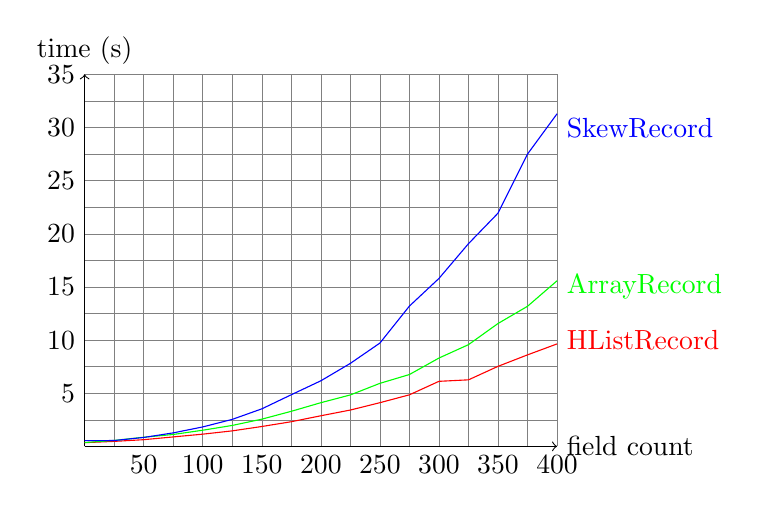
\begin{tikzpicture}[x=0.015cm,y=0.135cm]

  \def\xmin{0}
  \def\xmax{400}
  \def\ymin{0}
  \def\ymax{35}

  % grid
  \draw[style=help lines, xstep=25, ystep=2.5] (\xmin,\ymin) grid
  (\xmax,\ymax);

  % axes
  \draw[->] (\xmin,\ymin) -- (\xmax,\ymin) node[right] {field count};
  \draw[->] (\xmin,\ymin) -- (\xmin,\ymax) node[above] {time (s)};

  % xticks and yticks
  \foreach \x in {50,100,...,\xmax}
  \node at (\x, \ymin) [below] {\x};
  \foreach \y in {5,10,...,\ymax}
  \node at (\xmin,\y) [left] {\y};

  \draw[red] plot coordinates {
    (0  ,0.35)
    (25 ,0.47)
    (50 ,0.63)
    (75 ,0.89)
    (100,1.15)
    (125,1.46)
    (150,1.87)
    (175,2.32)
    (200,2.88)
    (225,3.42)
    (250,4.11)
    (275,4.85)
    (300,6.12)
    (325,6.26)
    (350,7.53)
    (375,8.61)
    (400,9.64)
   };
  \node[right,red] at (400, 10) {HListRecord};

  \draw[green] plot coordinates {
    (0  ,0.36)
    (25 ,0.56)
    (50 ,0.86)
    (75 ,1.12)
    (100,1.52)
    (125,1.97)
    (150,2.56)
    (175,3.30)
    (200,4.11)
    (225,4.84)
    (250,5.93)
    (275,6.76)
    (300,8.31)
    (325,9.57)
    (350,11.56)
    (375,13.18)
    (400,15.58)
  };
  \node[right,green] at (400,15) {ArrayRecord};

  \draw[blue] plot coordinates {
    (0  ,0.54)
    (25 ,0.55)
    (50 ,0.84)
    (75 ,1.27)
    (100,1.83)
    (125,2.54)
    (150,3.53)
    (175,4.86)
    (200,6.17)
    (225,7.81)
    (250,9.72)
    (275,13.20)
    (300,15.80)
    (325,19.07)
    (350,21.94)
    (375,27.50)
    (400,31.29)
  };
  \node[right,blue] at (400,30) {SkewRecord};

\end{tikzpicture}
\end{center}
\caption{Lookup: compile time}
\label{compile_time}
\end{figure}


\section{Conclusions and Future Work}\label{sec:conclusions}

Using type level programming techniques we developed two
new implementations of extensible records for Haskell: 
An array-like implementation, with constant time search and linear time insertion, and an impementation based on balanced trees that takes logarithmic time for searching and removing elements and constant time for
inserting elements. This run time performance is achieved by moving
most of the effort to compile time.

In the actual implementations we follow \cite{Leijen:scopedlabels} in allowing label repetition.  
A type-predicate \ensuremath{\Conid{HLabelSet}} can be added to disallow this as in \cite{KLS04}, with a slight cost in clarity but no cost in run time performance.

This approach can be used to improve the performance of systems
that make extensive use of extensible records. 
Some examples of such systems are the first-class attribute grammars library AspectAG \cite{FlyFirstClass}, 
the OOHaskell \cite{OOHaskell} library for object-oriented functional programming,
or libraries for relational databases such as CoddFish \cite{SV06} and HaskellDB \cite{haskelldb}.

Although the paper was focused on showing more efficient implementations of extensible records,
our aim was mainly to show how harnessing type level programming techniques it is possible
to improve the run time performance of some operations by moving certain computations to compile time.
Type level programming is commonly used to increase the expressivity and type safety of programs,
but in this paper we showed it can also be helpful for efficiency matters. 
This is the case specially for type level programming in Haskell, 
where there exists a phase distinction between compile and run time;
types are computed at compile time while values are computed at run time.

Interesting future work is to find a way to reduce compilation time.
Experiments demonstrate that GHC memoizes class instances,
but some particularity of our instances seem to confuse the mechanism.
\cite{PerfLeaks} suggests constraint reordering and striving for tail calls to improve
performance.
It did not work for us and it made the presentation less clear, so we went with the straightforward version. 

To improve performance, the code can be rewritten with type families. 
The main reason why we based our development on functional dependencies is the lack of overlapping instances at type families. 
In case further investigation on type families solves this problem we would be able to rephrase our implementation 
in terms of type families with a trivial translation, achieving a more functional style implementation.

An interesting aspect of the proposed approach to extensible records is that it can be encoded as a Haskell library, 
using only nowadays established extensions implemented for example in current versions of GHC.
However, better performance could be achieved if our approach is developed as a built-in implementation in a compiler. 
In that case, the \ensuremath{\Conid{ArrayRecord}} solution reduces to the standard tuple-based techniques \cite{Gaster96apolymorphic}.
On the other hand, \ensuremath{\Conid{SkewRecord}} provides a novel encoding with fast lookup and insertion that would preserve its advantages
even as a built-in solution.

\bibliographystyle{plainnat}

\begin{flushleft}
\begin{thebibliography}{24}
\providecommand{\natexlab}[1]{#1}
\providecommand{\url}[1]{\texttt{#1}}
\expandafter\ifx\csname urlstyle\endcsname\relax
  \providecommand{\doi}[1]{doi: #1}\else
  \providecommand{\doi}{doi: \begingroup \urlstyle{rm}\Url}\fi

\bibitem[Bazerman()]{PerfLeaks}
Gershom Bazerman.
\newblock Fixing performance leaks at the type level.
\newblock URL \url{http://www.haskell.org/pipermail/haskell-cafe/
  2011-July/093974.html}.

\bibitem[Bringert et~al.(2004)Bringert, H\"{o}ckersten, Andersson, Andersson,
  Bergman, Blomqvist, and Martin]{haskelldb}
Bj\"{o}rn Bringert, Anders H\"{o}ckersten, Conny Andersson, Martin Andersson,
  Mary Bergman, Victor Blomqvist, and Torbj\"{o}rn Martin.
\newblock {Student paper: HaskellDB improved}.
\newblock In \emph{Proceedings of the 2004 ACM SIGPLAN Workshop on Haskell},
  Haskell '04, pages 108--115. ACM Press, 2004.

\bibitem[Chakravarty et~al.(2005{\natexlab{a}})Chakravarty, Keller, and {Peyton
  Jones}]{1086397}
Manuel M.~T. Chakravarty, Gabriele Keller, and Simon {Peyton Jones}.
\newblock Associated type synonyms.
\newblock In \emph{ICFP '05: Proceedings of the tenth ACM SIGPLAN international
  conference on Functional programming}, pages 241--253, New York, NY, USA,
  2005{\natexlab{a}}. ACM.

\bibitem[Chakravarty et~al.(2005{\natexlab{b}})Chakravarty, Keller, {Peyton
  Jones}, and Marlow]{Chak05}
Manuel M.~T. Chakravarty, Gabriele Keller, Simon {Peyton Jones}, and Simon
  Marlow.
\newblock Associated types with class.
\newblock \emph{SIGPLAN Notices}, 40\penalty0 (1):\penalty0 1--13, January
  2005{\natexlab{b}}.

\bibitem[Gaster and Jones(1996)]{Gaster96apolymorphic}
Benedict~R. Gaster and Mark~P. Jones.
\newblock A polymorphic type system for extensible records and variants.
\newblock NOTTCS-TR 96-3, Nottingham, 1996.
\newblock URL \url{http://web.cecs.pdx.edu/\~{}mpj/pubs/polyrec.html}.

\bibitem[Hickey(2008)]{Hickey:2008:CPL:1408681.1408682}
Rich Hickey.
\newblock The clojure programming language.
\newblock In \emph{Proceedings of the 2008 Symposium on Dynamic Languages}, DLS
  '08, pages 1:1--1:1. ACM, 2008.

\bibitem[Hinze(2003)]{Hin03}
Ralf Hinze.
\newblock Fun with phantom types.
\newblock In Jeremy Gibbons and Oege {de Moor}, editors, \emph{The Fun of
  Programming}, pages 245--262. Palgrave Macmillan, 2003.

\bibitem[Hoogerwoord(1993)]{brauntrees}
Rob Hoogerwoord.
\newblock A logarithmic implementation of flexible arrays.
\newblock In R.~Bird, C.~Morgan, and J.~Woodcock, editors, \emph{Mathematics of
  Program Construction}, volume 669 of \emph{Lecture Notes in Computer
  Science}, pages 191--207. Springer Berlin / Heidelberg, 1993.

\bibitem[Jeltsch(2010)]{Jel10}
Wolfgang Jeltsch.
\newblock Generic record combinators with static type checking.
\newblock In \emph{Proceedings of the 12th international ACM SIGPLAN symposium
  on Principles and practice of declarative programming}, PPDP '10, pages
  143--154. ACM, 2010.

\bibitem[Jones and {Peyton Jones}(1999)]{Jones99lightweightextensible}
Mark~P. Jones and Simon {Peyton Jones}.
\newblock Lightweight extensible records for haskell.
\newblock In \emph{Proceedings of the 1999 Haskell Workshop}, {P}aris,
  {F}rance, October 1999.

\bibitem[Kiselyov(2012)]{type-eq}
Oleg Kiselyov.
\newblock {Type equality predicates: from OverlappingInstances to overcoming
  them}, 2012.
\newblock URL \url{okmij.org/ftp/Haskell/typeEQ.html}.

\bibitem[Kiselyov and L{\"a}mmel(2005)]{OOHaskell}
Oleg Kiselyov and Ralf L{\"a}mmel.
\newblock {Haskell's overlooked object system}.
\newblock Draft, 2005.

\bibitem[Kiselyov et~al.(2004)Kiselyov, L{\"a}mmel, and Schupke]{KLS04}
Oleg Kiselyov, Ralf L{\"a}mmel, and Keean Schupke.
\newblock {Strongly typed heterogeneous collections}.
\newblock In \emph{{Haskell '04: Proceedings of the ACM SIGPLAN workshop on
  Haskell}}, pages 96--107. ACM Press, 2004.

\bibitem[Leijen(2004)]{Leijen:fclabels}
Daan Leijen.
\newblock First-class labels for extensible rows.
\newblock Technical Report UU-CS-2004-51, Department of Computer Science,
  Universiteit Utrecht, December 2004.

\bibitem[Leijen(2005)]{Leijen:scopedlabels}
Daan Leijen.
\newblock Extensible records with scoped labels.
\newblock In \emph{Proceedings of the 2005 Symposium on Trends in Functional
  Programming (TFP'05)}, September 2005.

\bibitem[Myers(1983)]{Mye83}
Eugene~W. Myers.
\newblock An applicative random-access stack.
\newblock \emph{Information Processing Letters}, 17:\penalty0 241--248, 1983.

\bibitem[Okasaki(1996)]{OkaThesis}
Chris Okasaki.
\newblock \emph{Purely functional data structures}.
\newblock PhD thesis, Pittsburgh, PA, USA, 1996.
\newblock AAI9813847.

\bibitem[P.~Jones(2000)]{Jon00}
Mark P.~Jones.
\newblock Type classes with functional dependencies.
\newblock In \emph{ESOP '00: Proceedings of the 9th European Symposium on
  Programming Languages and Systems}, pages 230--244, London, UK, 2000.
  Springer-Verlag.

\bibitem[{Peyton Jones} and Morrisett(2003)]{LabeledFunctions}
Simon {Peyton Jones} and Greg Morrisett.
\newblock {A proposal for records in Haskell}, 2003.
\newblock URL \url{http://research.microsoft.com/en-us/um/people/simonpj/
  haskell/records.html}.

\bibitem[{Peyton Jones} et~al.(1997){Peyton Jones}, Jones, and Meijer]{PJM97}
Simon {Peyton Jones}, Mark Jones, and Erik Meijer.
\newblock Type classes: an exploration of the design space.
\newblock In \emph{Haskell Workshop}, June 1997.

\vfill
\eject


\bibitem[Schrijvers et~al.(2008)Schrijvers, {Peyton Jones}, Chakravarty, and
  Sulzmann]{Schrijvers2008}
Tom Schrijvers, Simon {Peyton Jones}, Manuel Chakravarty, and Martin Sulzmann.
\newblock Type checking with open type functions.
\newblock \emph{SIGPLAN Not.}, 43\penalty0 (9):\penalty0 51--62, September
  2008.

\bibitem[Silva and Visser(2006)]{SV06}
Alexandra Silva and Joost Visser.
\newblock Strong types for relational databases.
\newblock In \emph{Haskell '06: Proceedings of the 2006 ACM SIGPLAN workshop on
  Haskell}, pages 25--36, New York, NY, USA, 2006. ACM.
\newblock ISBN 1-59593-489-8.

\bibitem[Tullsen(2000)]{Tullsen00thezip}
Mark Tullsen.
\newblock The zip calculus.
\newblock In \emph{In Fifth International Conference on Mathematics of Program
  Construction (MPC 2000}, pages 28--44. Springer-Verlag, 2000.

\bibitem[Viera et~al.(2009)Viera, Swierstra, and Swierstra]{FlyFirstClass}
Marcos Viera, S.~Doaitse Swierstra, and Wouter Swierstra.
\newblock Attribute grammars fly first-class: how to do aspect oriented
  programming in haskell.
\newblock In \emph{Proceedings of the 14th ACM SIGPLAN international conference
  on Functional programming}, ICFP '09, pages 245--256. ACM, 2009.

\end{thebibliography}
\end{flushleft}

% \appendix

\end{document}

%%% Local Variables: **
%%% mode: latex **
%%% TeX-command-default: "LiterateHaskell" **
%%% TeX-master: t **
%%% TeX-default-extension: "lhs" **
%%% TeX-region: "_region_" **
%%% End: **

